\documentclass[output=paper]{langsci/langscibook}

\author{Nina Tahmasebi\affiliation{University of Gothenburg} and
Lars Borin\affiliation{University of Gothenburg} and
Adam Jatowt\affiliation{University of Innsbruck}} 

\title{Survey of computational approaches to lexical semantic change detection}

\abstract{Our languages are in constant flux driven by external factors such as cultural, societal
and technological changes, as well as by only partially understood internal motivations. Words acquire new meanings and
lose old senses, new words are coined or borrowed from other languages
and obsolete words slide into obscurity. Understanding the
characteristics of shifts in the meaning and in the use of words is useful for those who work with the content of historical
texts, the interested general public, but also in and of itself. 

The findings from automatic lexical semantic change detection, and the models of diachronic conceptual change are also currently being incorporated in approaches for measuring document across-time similarity, information retrieval from long-term document archives, the design of OCR algorithms, and so on. In recent years we have seen a surge in interest in the academic community in computational methods and tools supporting inquiry into diachronic conceptual change and lexical replacement.
This article provides a comprehensive survey of recent computational techniques to tackle both.}
  
\begin{document}
\maketitle

\section{Introduction}\label{sec:intro}

Vocabulary change has long been a topic of interest to linguists and the general public alike. This is not surprising  considering the central role of language in all human spheres of activity, together with the fact that words are its most salient elements. Thus it is natural that we want to know the ``stories of the words we use'' including when and how words came to possess the senses they currently have as well as what currently unused senses they had in the past. And while some examples are commonly known, like \textit{gay} having meant 
`happy' in the past, the fact that \textit{girl} used to mean `young person of either gender' is unknown to many. Professionals and the general public are interested in the origins and the history of our language as testified to by numerous books on semantic change aimed at a wide readership.

\begin{sloppypar}
Traditionally, vocabulary change has been studied by linguists and other scholars in the humanities and social sciences with manual, ``close-reading'' approaches. While this is still largely the case inside linguistics, recently we have seen proposals, originating primarily from computational linguistics and computer science, for how semi-automatic and automatic methods could be used to scale up and enhance this research.
\end{sloppypar}

Indeed, over the last two decades we have observed a surge of research papers dealing with detection of lexical semantic changes and formulation of generalizations about them, based on datasets spanning decades or centuries. With the digitization of historical documents going on apace in many different contexts, accounting for vocabulary change has also become a concern in the design of information systems for this rapidly growing body of texts. At the same time, as a result, large scale corpora are available that allow the testing of computational approaches for related tasks and that provide quantitative support to proposals of various hypotheses.\largerpage

Despite the recent increase in research using computational approaches to investigate lexical semantic changes, the community is in critical need of an extensive overview of this growing field. The aim of the present survey is to fill this gap. While we were preparing this survey article, two related surveys appeared, illustrating the timeliness of  the topic.\footnote{This survey is an updated and published version of the survey presented by \citet{tahmasebi2018survey}.} The survey by \citet{kutuzov-etal-2018-diachronic} has a narrower scope, focusing entirely on diachronic word embeddings. The broader survey presented by \citet{tang-2018} covers much of the same field as ours in terms of computational linguistics work, but provides considerably less discussion of the connections and relevance of this work to linguistic research. A clear aim in preparing our presentation has been to anchor it firmly in mainstream historical linguistics and lexical typology, the two linguistic subdisciplines most relevant to our survey. Further, the application of computational methods to the study of language change has gained popularity in recent years. Relevant work can be found not only in traditional linguistics venues, but can be found in journals and conference proceedings representing a surprising variety of disciplines, even outside the humanities and social sciences. Consequently, another aim of this survey has been to provide pointers into this body of research, which often utilizes datasets and applies methods originating in computational linguistics research. Finally, our main concern here is with computational linguistic studies of vocabulary change utilizing empirical diachronic (corpus) data. We have not attempted to survey a notable and relevant complementary strand of computational work aiming to simulate historical processes in language, including lexical change (see \citealp{baker-2008} for an overview). We also leave out of consideration work utilizing digitized historical dictionaries as the primary data source \citep[e.g.,][]{xu2017evolution,ramiro2018,cathcart-2020}. While historical text digitization initiatives are often undertaken by public cultural heritage institutions such as national libraries, historical dictionaries are as often as not commercial ventures which makes them both very scarce and often not freely accessible in a way which would allow reproducibility of experiments, let alone release of enriched versions of the dictionaries.\footnote{For instance, according to the website \url{https://ht.ac.uk/terms/}, accessed April 4th, 2021, the \emph{Historical Thesaurus of English} that was used for the studies of \citet{xu2017evolution} and \citet{ramiro2018} is available for research by agreement only and only on quite specific conditions, to a limited number of research projects at the same time.}

The work surveyed here falls into two broad categories. One is the modeling and study of \textsc{diachronic conceptual change} (i.e., how the meanings of words change in a language over shorter or longer time spans). This strand of computational linguistic research is closely connected to corresponding efforts in linguistics, often referring to them and suggesting new insights based on large-scale computational studies, (e.g., in the form of ``laws of semantic change''). This work is surveyed in two sections, 
one section on word-level change in Section~\ref{sec:wsch}, and one on sense-differentiated change in Section~\ref{sec:sdcd}. The word-level change detection considers both count-based context methods as well as those based on neural embeddings, while sense-differentiated change detection covers models based on topic modeling, clustering, word sense induction,  and -- the most recent development -- contextualized embeddings.\largerpage

The other strand of work focuses on \emph{lexical replacement}, where different words express the same meaning over time. This is not traditionally a specific field in linguistics, but it presents obvious complications for access to historical text archives, where relevant information may be retrievable only through an obsolete label for an entity or phenomenon. Because successful approaches to semantic change over longer time scales are strongly dependent on the possibility to first resolve lexical replacements, we cover this body of work in Section~\ref{sec:dwr}. 


The terminology and conceptual apparatus used in works on lexical semantic change are multifarious and not consistent over different fields or often even within the same discipline. For this reason, we provide a brief background synopsis of relevant linguistic work
 in Section~\ref{sec:lingappr}.

Much current work in computational linguistics depends crucially on (formal, automatic, quantitative, and reproducible) \textsc{evaluation}. Given the different aims of the surveyed research, evaluation procedures will look correspondingly different. We devote Section~\ref{sec:method} to a discussion of general methodological issues and evaluation.


We end with a summary of the main points garnered from our literature survey, and provide a conclusion and some recommendations for future work (Section~\ref{sec:summary}).

We believe our survey can be helpful for both researchers already working on related topics as well as for those new to this field, for example, for PhD candidates who wish to quickly grasp the recent advances in the field and pinpoint promising research opportunities and directions. 


\section{Linguistic vs. computational approaches to vocabulary change}\label{sec:lingappr}
\subsection{Terminological and conceptual prelude}\label{sec:lingterms}
The study of how meaning -- including lexical meaning -- is
expressed and manipulated in language is pursued in a number of
scientific disciplines, including psychology, (cultural) anthropology,
history, literature, philosophy, cognitive science, and in linguistics
and computational linguistics. These all construe the problems
involved in studying linguistic meaning in different ways, for
different purposes, and consequently conceptualize this field of
inquiry differently, with concomitant differences in
terminology. Drawing on partly common origins, they unfortunately
often use the same terms, yet with different meanings.

Our primary frame of reference in this chapter is provided
by relevant work in (general) linguistics, being the field offering
the theoretically and empirically best-grounded view on the phenomena
under discussion here. In particular, in studying meaning in language,
linguistics takes a broad cross-linguistic perspective, which is typically
lacking in the other disciplines addressing this question.

Because many of the terms found in discussions of lexical change are not used in the same way by all authors, we start out by defining our use of some central terms. In order to discuss linguistic
semantics and semantic change over time, we need to distinguish the following notions. \textsc{linguistic form} or
\textsc{linguistic substance} is the physical manifestation of language:
linguistic expressions formed using sound, writing, or sign(ed
language). In addition, linguistic form is normally taken to include certain
structural aspects of language expressions, such as parts of speech,
inflectional paradigms, dependency trees, and so on. \textsc{meaning} or
\textsc{sense} is information -- in a wide sense -- conventionally connected with (or conveyed
by) the forms. It is essentially thought of as something residing in
the minds of the language users. The sense is what a dictionary
definition aims to capture. Linguistic meaning is generally considered
to exhibit at least two aspects. \textsc{denotation} or \textsc{denotative
  meaning} corresponds to the ``neutral'' information content. 
\textsc{connotation} or \textsc{connotative meaning} refers to attitudinal
or sentiment-conveying aspects. The English words \emph{thrifty} and
\emph{stingy} have by and large the same denotation but different
connotations.

Finally, linguistic meaning connects language to the extralinguistic
realm: to the actual world and also to imagined situations. Here, the
terminology becomes more motley, and for our purposes in this chapter
it will suffice to note that the relation of linguistic meaning to
extralinguistic reality can be seen as indirect~-- mediated by mental
\textsc{concepts}\footnote{Some authors make no distinction between
  ``meaning'' and ``concept'', and both terms unfortunately have many
  -- sometimes mutually incompatible -- uses in the literature. ``Concept'' is
  especially treacherous, since it is treated -- sometimes explicitly
  defined -- as a term, but with widely differing content in different
  contexts. E.g., the ``concepts'' of conceptual historians seem to
  actually be simply words, reflected in statements about the
  ``changing meaning of concepts'' \citep{richter-1996}, which makes
  their undertaking tantamount to (a kind of) etymological study. We
  will use the two terms -- sparingly -- interchangeably here, with
  the understanding that neither term is well-defined.} -- or direct --
the case of proper nouns, which refer directly.  The main function of
a personal name like \emph{Faith} is to pick out an individual and the
fact that the word also corresponds to a common noun is of no import
in this case,\footnote{Thus, the personal name \emph{Faith} will not
  be ``translated'' into Russian \emph{Vera} or Finnish \emph{Usko},
  both of which in addition to being personal names are also common
  nouns literally meaning `faith, belief' (and the Finnish
  correspondent is actually a male name).} and does not help us
identify the individual in question.

Students of human linguistic behavior and language have been
investigating and discussing the nature of these notions and their
relationships for millennia, so this brief introduction cannot do
justice to all the complexities involved. Rather, we have tried to
summarize briefly what we understand as a view broadly shared among
linguists, and only to the extent necessary for the present survey.


In this chapter, the linguistic forms in focus are \textsc{lexical
  items}, i.e., words (or multiword expressions) that are not
\emph{semantically} decomposable into smaller parts.\footnote{Although they will often be \emph{formally} decomposable, the semantics of the whole is not computable from that of the parts.} Among the lexical items
we also include proper nouns and function words. Interchangeably with
lexical item we will also say ``word'', intending this term also
to apply to multiword expressions.

Note that lexical items are not the same thing as \textsc{text
  words}. A lexical item in our usage of this term corresponds roughly
to what is often called \textsc{lexeme} in lexicography
\citep[e.g.,][]{matthews-1974}, basically what we understand as an entry
-- a word or multiword expression -- in a conventional dictionary,
referring through a \textsc{citation form} or \textsc{lemma} to a
bundle of formal characteristics, including at least a part of speech
and possibly a set of inflected forms, which make up the text words
subsumed by the lexical item. The inflectional pattern, while an
important clue to lexemehood in many languages, is not so salient in
English, where generally lemma and part of speech are sufficient to
uniquely identify a lexical entry, but an example could be
\emph{stick} (v).  It corresponds to two such lexical units: one with
the past form \emph{stuck} `to pierce, to fasten, etc.' and another
with the past form \emph{sticked} `to furnish (a plant, vine, etc.)
with a stick or sticks in order to prop or support'. Another example: \emph{die}
(n), with the plural form \emph{dies} `a cutting or impressing tool'
or \emph{dice} `small cube with numbered sides used in games'.

We will refer to the combination of a lexical item and a particular
recognized meaning of that lexical item as a \textsc{word sense}. Thus,
both \emph{bank} (n) `(a kind of) financial institution' and
\emph{bank} (n) `extended shallow portion of sea or river floor' are word
senses according to this definition, as are \emph{moose} (n) `a kind of
(game) animal' and \emph{moose} (n) `meat of this animal used as food'.

The relationship between forms and meanings is many-to-many, so
one form may be used to express more than one meaning, and, conversely, the same meaning can be expressed by more than one form. The
former configuration will be consistently referred to as
\textsc{polysemy} (or \textsc{colexification}\footnote{This is a more neutral term often encountered in the lexical typological literature intended to cover both polysemy and homonymy \citep[e.g.,][]{francois2008semantic,ostling-2016}.}) even when some lexicographical traditions
would distinguish it from \textsc{homonymy}. This distinction is hard
or impossible to make categorically
\citep{apresjan-1974,murphy-2003,riemer-2010,wishart-2018}, so we have not attempted to make it.\footnote{According to
  \citet{apresjan-1974} we should recognize polysemy (as opposed to
  homonymy) when two senses of a word exhibit non-trivial common
  components in their definitions. However, he does not discuss how to ensure
  intersubjective agreement on definitions, which makes this
  criterion less than exact. Similarly for the ``technical definition
  of concept'' (where ``concepts'' correspond to homonymous -- main --
  senses of a lexeme) provided by \citet[235; emphasis in the
    original]{cooper05}: ``Two meanings of a given word correspond to
  the same \emph{concept} if and only if they could inspire the same
  new meanings by association.'' Again, there is no indication in the
  article of how this definition could be operationalized to ensure
  intersubjective agreement. This is not to deny that lexeme meanings
  can be seen as hierarchically organized or that the intuitions
  behind the cited statements are well-founded, but simply to
  recognize that there are no straightforwardly applicable mechanical
  criteria for distinguishing polysemy from homonymy, and also --
  which Apresjan acknowledges -- that in reality this is not a
  dichotomy, but rather a cline. Consequently, some of the methods
  discussed in this survey article could in fact be applied also to
  the problem of teasing out hierarchical relationships among word
  senses of the same lexeme.}  The latter configuration is known as
\textsc{(near) synonymy}, and, depending on its definition in a
particular lexicographical tradition, it may be seen as frequent (as
in a wordnet) or next to non-existent
\citep{cruse-1986,ci-2008,murphy-2003,riemer-2010}.

While the form units -- the words -- are comparatively easy to
identify in language, word senses are notoriously difficult to
isolate. Much of the work surveyed in this chapter takes a published
lexicon as providing the canonical sense set, the gold standard by
which to judge system accuracy. While this is a practical solution for
many purposes, it also, in effect, ignores a host of difficult
theoretical and methodological questions. For the purposes of this
survey, we do not take a stand on precisely how word senses are
defined and identified, but we do note that some of the approaches
represented in the surveyed work have the potential to throw light on
these questions; see below.

\subsection{Linguistic studies of lexical change}
To a linguist, the topic of this chapter would fall under the
rubric of \textsc{historical-comparative linguistics} or
\textsc{diachronic linguistics}. This is a branch of general linguistics that
concerns itself with how languages change over time and with
uncovering evidence for genetic relations among languages
\citep{anttila-1972,campbell,hl-handbook}. This linguistic subfield
has a long history, antedating by a century or so the birth
of modern \textsc{synchronic linguistics}. The latter by and large emerged in
the early twentieth century in no small measure as a reaction against
the predominant historical orientation of mainstream linguistics of the time.

Even if now relegated to a more modest position within the
language sciences, historical-comparative linguistics is very
much alive and an active branch of linguistic research. For this
reason it is interesting to elucidate how it interacts, or could
interact, with the computational linguistics research surveyed here.

\subsubsection{Lexical change, semantic change, grammaticalization, and lexical replacement}

The phenomena addressed in the works surveyed in this chapter
(i.e., historical developments in the vocabulary of a language or languages) are
studied by historical linguists under the headings of \textsc{lexical change}, \textsc{semantic change}, \textsc{grammaticalization}, and \textsc{lexical replacement}.

In linguistic literature, the term lexical change unfortunately is used in two senses. In the sense  used here, it is a general cover term for all kinds of diachronic changes in the vocabulary of a language or languages. The other common usage is a hyponym of this, referring to new forms entering or leaving the language, i.e., loanwords and
neologisms of various kinds, and obsolescing words, respectively. 

Lexical replacement refers to a lexeme being ousted by another synonymous lexeme over time, as when \emph{adrenaline} is replaced by \emph{epinephrine}. 
A particular form of
lexical replacement which has received a fair amount of attention in
computational linguistics but which is generally not studied at all by
historical linguists is \textsc{named entity change}.\footnote{This is most likely because, strictly speaking, named entity change
does not involve word senses at all (see above). However, the \emph{etymology} of names -- in particular place names -- plays
  an important role in historical linguistics, where it is studied under the label of \textsc{toponymy}, as a clue to
  determining prehistorical linguistic geography and population
  movements. For example, the fact that the city names \emph{Dresden} and
  \emph{Leipzig} both have a recognizable Slavic origin is taken to
  confirm a more westerly extension of Slavic speakers in earlier
  times in present-day Germany. This is also indicated  by historical records. It is also true that names can be the basis for general vocabulary, in other words, the etymology of a non-name must sometimes make reference to a name. For example, \emph{bedlam}, from the (nick)name of a psychiatric hospital in London, or the (Chilean) Spanish verb \emph{davilar} `to botch things up royally', from the surname of Juan Pablo Dàvila, an infamous spectacularly inept financial trader (\url{https://www.improbable.com/ig/winners/\#ig1994}). Finally, a cultural taboo against naming the dead may lead to avoidance of words sounding like the name of a recently deceased person, replacing them with, e.g., loanwords \citep[8f]{alper-nash-1999}.}

Semantic change or semantic shift is the normal term for the special case of lexical
change where an existing form (a lexeme) acquires or loses a particular meaning,
i.e., increasing or decreasing polysemy
\citep{traugott2001regularity,fortson-2003,newman-2016,traugott-2017}. An example are the oft-cited changes whereby on the one hand an earlier English word for a
particular kind of dog became the general word for `dog', and,
on the other, the earlier general word for `dog' -- whose modern reflex
is \emph{hound} (n) -- is now used for a special kind of dog.

There are two complementary approaches adopted by linguists to
the study of the lexicon. Lexical items can be studied from the
\textsc{onomasiological} point of view, investigating how particular
meanings (or concepts) are expressed in a language. The Princeton
WordNet \citep{fellbaum-1998} is an onomasiologically organized
lexical resource, as is, e.g., \emph{Roget's Thesaurus}
\citep{roget-1852}.  The more common \textsc{semasiological} approach
takes linguistic forms -- words and multiword expressions -- as its
point of departure and investigates which meanings they express. Conventional dictionaries are semasiologically organized.

\begin{sloppypar}
Studies of semantic change adopt the semasiological perspective, whereas works on other forms of lexical change generally have an onomasiological focus.
\end{sloppypar}

Grammaticalization
\citep{hopper-traugott-1993,heine-kuteva,smith-2011} denotes a
particular kind of semantic change, where content words turn into
function words and ultimately into bound grammatical morphemes. One example is the
French preposition \emph{chez} `at, with', developed from the Latin
noun \emph{casa} `(small) house, cottage'.\footnote{See
  \url{http://www.cnrtl.fr/definition/chez}.}

In both semantic change and grammaticalization, the form is thus fixed
-- modulo historical sound shifts\footnote{That is, Latin \emph{casa}
  and French \emph{chez} count as the same word, even though they do
  not in fact share a single speech sound (\emph{casa} sounded more or
  less as expected -- 
  [ˈkasa] 
-- while \emph{chez} is pronounced 
  [ʃe]), 
  since the
  latter is derived from the former by regular historical sound
  changes.} -- while its content changes.

The term \textsc{etymology} refers to the scientific investigation of the origin and history of
lexical items, whose development may include both onomasiological and
semasiological aspects \citep{malkiel,anttila-1972,mailhammer-2015}. In fact, these
aspects interact in a natural way, and are perhaps best thought of as
different views on a unitary phenomenon, viz. lexical change. 

\subsubsection{Theoretical and methodological aspects of the linguistic study of lexical change} 

A central activity in the linguistic study of vocabulary change is the description of individual
changes in the vocabulary of a language or group of related
languages. The concrete outcome of this research is the etymological
article or dictionary.

As its name indicates, general linguistics studies language as a
universal phenomenon, and collecting data about individual languages
is thought of as contributing to this goal. Consequently, an important
concern of this field of inquiry is the generalization of sets of
observed individual lexical changes into types and classes of changes,
valid for human languages in general. This includes uncovering
universal or general directional tendencies -- ``laws'' -- of semantic
change, such as person-part $>$ enclosing person-part (e.g.,  `mouth' $>$
`face'), but not the opposite \citep{wilkins}, many individual
grammaticalization paths and, more generally, the assumed
unidirectionality of grammaticalization
\citep{heine-kuteva,smith-2011}.

The common event of adding a word sense to the vocabulary of a
language can be accomplished in several different ways. These are, by
borrowing, coining a new word \emph{ex nihilo} (rare) or using the
word-formation machinery of the language, or finally -- and commonly
-- adding a word sense to an existing lexeme. The latter can again be
achieved by, for example, \textsc{generalization} or
\textsc{broadening} (English \emph{dog} `a kind of dog' $>$
`dog')\footnote{Generalization is also considered to make up an
  important initial stage of grammaticalization \citep{smith-2011}.}
and \textsc{specialization} or \textsc{narrowing} (English
\emph{hound} `dog' $>$ `a kind of dog'). Other types of semantic
change have their origin in \textsc{metaphor}, as in the \emph{foot}
of a mountain or the \emph{head} of a state; in \textsc{metonymy}, for
example, the development where \emph{bead}, a word originally meaning
`prayer', acquired its current meaning from the use of a rosary while
praying; and in \textsc{ellipsis}, as \emph{mobile} and \emph{cell} from
\emph{mobile phone} and \emph{cell phone}, respectively. For a more detailed oveview of (lexical) semantic change and how this phenomenon has been studied by linguists, see
\citet{urban-2015}. Finally, a lexeme in one language may add a sense
by mirroring a polysemy in another language, a form of loan
translation. For example, the Swedish verb \emph{suga} `to suck' has
acquired a recent new sense `to be unpleasant, inferior, etc.'
borrowed from English. From this it follows that semantic change
typically involves polysemy or colexification. Crucially, even cases
of seemingly complete sense change in a lexeme are thought to involve
an intermediate (unattested) polysemous stage: A $>$ A+B $>$ B, or A~$>$ 
A+b $>$ a+B $>$ B, where A/a and B/b are senses related by some
regular mechanism of sense change and caps indicate a dominant
sense. Thus, variation in the language community in the distribution
of these colexified senses is what ultimately drives semantic change
\citep{bowern2019semantic}.\largerpage

The activities of broadly characterizing and classifying vocabulary
changes overlap significantly with another linguistic subdiscipline,
namely \textsc{lexical typology}
\citep{k-tamm-2008,k-tamm-2012,k-tamm-etal-2016}. This is also
referred to as \textsc{semantic typology} \citep{riemer-2010}, whose
aims are to elucidate questions such as ``how languages categorize
particular domains (human bodies, kinship relations, colour, motion,
perception, etc.) by means of lexical items, what parameters underlie
categorization, whether languages are complete\-ly free to ``carve up''
the domains at an infinite and arbitrary number of places or whether
there are limits on this, and whether any categories are universal
(e.g., `relative', `body', or `red')''
\citep[434]{k-tamm-etal-2016}. These questions are relevant to
classificatory activities, since universal restrictions on or
tendencies of lexicalization will determine which semantic changes are
possible or likely, as opposed to impossible or unlikely.

However, as \citet[148]{anttila-1972} observes, ``labeling
before-after relations [\ldots] does not explain anything; it just
states a fact'', and a central goal of linguistics is to explain
linguistic phenomena. Hence, a third kind of activity is the
search for enabling factors and, ultimately explanations for the
observed changes and regularities of change formulated on the basis of
broad cross-linguistic comparison.

In their search for explanations of lexical change, linguists have
proposed some factors that seem to play a role in lexical change,
as (proximal or distal) causes or as enabling or constraining
mechanisms. Material and immaterial culture are almost always
mentioned in this connection. In order to be able to talk about new
objects, phenomena, and practices, we need new vocabulary, so the argument goes. At one point, historical linguists saw this as a -- or even the -- major
driving force behind lexical change, a point of view forcefully
argued by the \emph{Wörter und Sachen} `words and things'
school active at the beginning of the 20th century
\citep{meringer-1912}.

Other potentially influencing factors, which have been discussed in
the linguistic literature, are human physiological and cognitive
characteristics (e.g., in relation to color vocabulary), systematic
sound symbolism/onomatopoeia \citep{erben-johansson-etal-2020}, the
size of the language community, language contact, and the presence of
large numbers of L2 speakers, among others. For example,
\citet{ellison-miceli-2017} adduce linguistic and psycholinguistic
evidence that bilinguals speaking closely related languages develop a
cognitive bias against recognizably shared word forms \citep[termed
  ``doppels'' by][]{ellison-miceli-2017}, which they argue accelerates
lexical change.


\subsection{Historical-comparative linguistics meets computational linguistics?}

When historical linguists started to use computers more than half a
century ago, their primary focus was initially on modeling sound
change as formal rule systems, in order to check that postulated
changes yield the expected outcome, or to reverse the changes to
produce putative proto-forms from modern forms
\citep[e.g.,][]{hewson-1973,hewson-1974,johnson-1985,borin-1988,lowe-mazaudon-1994}. In
more recent times and coinciding with the statistical and
machine-learning emphasis characterizing present-day computational
linguistics, massively multilingual datasets have been employed for
genealogical classification of languages \citep{brown-etal-2008}.

In the  linguistic subfield of corpus linguistics,\footnote{Corpus linguistics is related to computational linguistics but often surprisingly
separate from it. The two fields do share an interest in applying computational methods to language, but at the same time they differ crucially in their primary aims.} the
increasing availability of large historical text sets has spurred
corpus-based work on historical semantics and pragmatics
\citep{ihalainen-2006,taavitsainen-fitzmaurice-2007,allan-robinson-2011}. 
This
work is typically semasiological and particularistic in spirit, taking
as its point of departure particular words -- given a priori -- and
endeavoring to track their shifting semantics over time
\citep[e.g.,][]{sagi-etal-2011,kerremans-etal-2011}. The only efforts
we are aware of in this area to address the problem in a more general
way do so only indirectly. \citet{koplenig-2017} and \citet{degaetano2017diachronic}, for example, describe computational 
methods for identifying changing word usages over time in
diachronic text, but it
is reasonable to assume, ceteris paribus, that these changes often (or always) will
reflect changing semantics of the forms thus identified.

While some of the work described and discussed in the present survey
has not been directly motivated by linguistic research questions, the
authors of these works often indicate the potential usefulness of
their results to linguistics. We believe that computational approaches
to lexical and semantic change have the potential to provide a
genuinely novel direction for historical linguistics.  However, this
is not likely to happen without these authors paying more attention to
the theoretical and methodological assumptions of current historical
linguistics, an awareness sometimes lacking in the work surveyed. For
linguists to take notice of this work, it needs to show awareness of
the state of the art of diachronic linguistics and argue in terms
understandable to a linguistic audience.

In this connection, a central methodological question will be
\textsc{representativeness}. During the rapid growth phase of corpus linguistics in the 1970s and
1980s, representativeness was a much discussed concern
\citep[e.g.,][]{atkins-etal-1992,biber-1993,clear-1993,johansson-1994},
the issue of course being the question if we will be able to say anything meaningful about our actual object of study,
the language,  when investigating the
corpus. The question remains, but tends to be rarely addressed
in the computational linguistics literature, one notable exception being the work of \citet{koplenig2016,koplenig-2017}.

In diachronic studies, the demands for representativeness are
exacerbated by the requirement to compare two or more temporal
language stages. We must ensure that all investigated time-slice
subcorpora are equally representative of their respective language
stages. Linguistic differences between the subcorpora must not be
caused by some confounding extralinguistic factor. An example may make
this more concrete. \citet[Ch. 4]{underwood-2019} -- a literary
scholar -- presents a study of ``gendered language'': words used to
portray feminine and masculine characters in English-language fiction
in the period 1840--2000. First, and importantly to our example, the
study shows that there are clear demonstrable differences in terms of
the words used by authors for depicting masculine and feminine
characters and their actions, although the differences grow smaller
over the course of the twentieth century. However, the study also
reveals some relevant additional facts, namely
\begin{itemize}
\item ``a fairly stunning decline in the proportion of fiction writers who were women from the middle of the nineteenth century to the middle of the twentieth [\ldots] from representing almost half the authors of fiction to less than a quarter'' \citep[133]{underwood-2019}; and
\item that over the same period, ``[w]omen are constantly underrepresented in books by men'' \citep[127]{underwood-2019}.
\end{itemize}

These two facts together could lead to words used specifically to
describe feminine characters exhibiting a significant shift in
distribution over time in such a diachronic fiction material, which
could be interpreted as semantic change.

On the other hand, the most crucial awareness is simply this:
``Knowing that your corpus is unbalanced is what counts. It would be
shortsighted indeed to wait until one can scientifically balance a
corpus before starting to use one, and hasty to dismiss the results of
corpus analysis as `unreliable' or `irrelevant' simply because the
corpus used cannot be proved to be `balanced'.''
\citep[6]{atkins-etal-1992}. In particular with historical data, it may
not even be possible to achieve balance in the sense expected from a
modern corpus.

As discussed above, lexical change can be seen as a special case of
lexical variation, which in turn can be attributable to many different
linguistic and extralinguistic factors. In other words, we see the
task of establishing that we are dealing with variants of the same
item (in some relevant sense) -- items of form or content -- as
logically separate from -- and logically prior to -- establishing that
the variation is classifiable as lexical change.

Investigation of lexical change is further complicated by the fact
that -- as just noted -- observed variation in lexical form between
different text materials need not be due to diachronic causes at all,
even if the materials happen to be from different time
periods. Linguists are well aware that even seen as a synchronic
entity, language is full of variation at all linguistic levels. In
spoken language, this kind of variation is the norm. Words have a wide
range of pronunciations depending on such factors as speech rate,
register/degree of formality, phonetic and phonological context,
etc. If the language has a written form, some of this variation may be
reflected in the orthography, but orthography may also reflect
ambiguous principles for rendering some sounds in writing, as when /s/
can be written alternatively (at least) with 〈s〉, 〈c〉, 〈z〉 and 〈ps〉 in
Swedish. Spelling principles -- if standardized at all, which often is
not the case in older texts -- may change over time independently of
any changes in pronunciation (``spelling reforms''), and in such
situations written texts may exhibit a mix of the older and newer
orthography. Finally, in many modern text types we find a large number
of spellings which deviate from the standard orthography
\citep{eisenstein-2015}.

A fundamental question underlying all work on semantic change is the
problem of identifying like with like, or -- on the form side --
classifying text words under relevant lexical units, and -- on the
content side -- identifying and grouping relevant senses.

Although often trivial, even the former task is complicated by the
existence of multiword expressions, the need for word segmentation (in
speech and some writing systems), and -- a fortiori in a
diachronic context -- language variation, which may be purely
orthographic, both synchronically and diachronically, as well as a
reflection of sound change in the diachronic setting.\footnote{Orthography interacts in intricate ways with language change. Since spelling is often conservative, it may provide hints about earlier, pre-sound change forms of words, such as written-word initial 〈kn-〉 in English (e.g., \emph{knight}), which may help us to see connections among lexical items which have otherwise been obscured by sound change. A (sporadic) case such as English 〈discreet〉 vs. 〈discrete〉 -- where two spelling variants of the same original item (still pronounced identically) parted ways in the late 16th century  (\url{https://www.dictionary.com}, s.v. \emph{discreet}) -- will serve as concrete evidence of polysemy, although not of course in an exclusively written-language setting.} 

The latter task is widely recognized to be unsolved, and possibly not
even amenable to finding one solution in that there will not be one
canonical sense set for a particular language, but several sets
depending both on their intended use \citep{kilgarriff1997}, on
particular analytical traditions (``lumpers'' vs. ``splitters''), and
even on individual idiosyncrasies.\footnote{Or on completely
  extraneous factors, such as budget constraints \citep{lange-2002}.}
In this context work such as that surveyed here can make a real
contribution, by putting the identification of senses on a much more
objective footing, and also allow for different sense granularities
for different purposes by adjusting model parameters \citep{erk-2010}.

On a more basic level, these questions are intimately related to some
of the basic theoretical and methodological conundrums of linguistics,
such as the nature of words
\citep{aikhenvald-dixon-2002,haspelmath-2011}, of concepts
\citep{murphy-2002,wilks-2009,riemer-2010} and their relation to word
senses \citep{cruse-1986,kilgarriff1997,kilgarriff-2004,hanks-2013}.

Generally speaking, training in (historical) linguistics prepares
researchers to take such confounds and caveats into account, giving
them a fair idea of which the crucial non-relevant variables are
likely to be, and, importantly, how to design investigative procedures
which ``short-circuit'' such variables. Lack of such training of
course comes with the risk that experiments will be poorly designed or
their results misinterpreted.

In the final count, however, the computational methods surveyed in
this chapter represent a genuinely novel approach to addressing many
research questions of historical linguistics, and linguists must be
prepared to assimilate the methods at least to some extent in order to
grasp the implications of the results. Thus, if these methods are to
make an impact on research in historical linguistics -- as we think
they could -- a conceptual shift is most likely required in both
camps.

\subsection{Computational studies of lexical change: A classification}

Relating the main kinds of lexical change which have been considered in computational linguistics to those discussed in historical linguistics, we note that there is no neat one-to-one correspondence. The study of \emph{semantic change} looms large in both fields and by and large focuses on the same kinds of phenomena, but in computational work, this is typically combined with a study of gain and loss of lexemes (i.e., \emph{lexical change} in the narrower sense), since these phenomena are uncovered using the same computational methods. This could be said to constitute a consistent focus on the conceptual side of the vocabulary, which however is not normally present in historical linguistics and consequently not given a label. In this survey, we refer to it as \textsc{diachronic conceptual change}, i.e. change in the set of lexical meanings of a language. We propose this term as a superordinate concept to semantic change. Diachronic conceptual change takes the view of all senses and word-sense allocations in the language as a whole. This includes a new word with a new sense (e.g., neologisms like \emph{internet} with a previously unknown sense) as well as an existing word with a new sense (\emph{gay} firstly receiving a `homosexual' sense, and later more or less losing its `cheerful' sense), because both of these add to the set of senses available in the language. Diachronic conceptual change also allows for changes to the senses themselves, the line between actual meaning change and usage change is blurry here. Examples include the \emph{telephone} that is a `device for conveying speech over a distance', but that is now also used for spread of communication, and increasingly as a `personal device used for photography, scheduling, texting, working', and so on. 

Further, the specific phenomena of \emph{lexical replacement} (including \emph{named entity change}) and its generalized version \textsc{temporal analogy} have been subject to many computational linguistic studies.  Examples include the placename \emph{Volgograd} that replaced \emph{Stalingrad}, which in its turn earlier had replaced \emph{Tsaritsyn} (named entity change), \emph{foolish} that replaced \emph{nice} for the `foolish' sense of the latter word (lexical replacement), and \emph{iPod} that can be seen as a temporal analog of a \emph{Walkman}.
The change classes and their ordering as they are being studied from a computational perspective are shown in Table \ref{tab:changetypes-v2}, and different types of semantic change are shown in Table \ref{tab:changetypes}.

\begin{table}[H]
\caption{Change types and their organization considered from a computational perspective }\label{tab:changetypes-v2}
\fittable{\begin{tabular}{ll}  
\lsptoprule
\multicolumn{2}{c}{Lexical semantic change} \\
\midrule
Lexical change  &   Diachronic conceptual change\\
\cmidrule(r){1-1}
\cmidrule(r){2-2}
Lexical replacement &  Semantic change (new allocation of existing words and senses)\\
Named Entity change &  New word senses allocated to an existing word\\
Role changes &  New words with completely new word sense\\
Temporal analogy &  New word with a new but existing sense\\
& Changes to existing senses\\
\lspbottomrule
\end{tabular}}
\end{table}


\begin{table}[H]
 \caption{Change types investigated in the surveyed literature (ws = word sense)}\label{tab:changetypes}
 \fittable{\begin{tabular}{ll}
\lsptoprule
Change type & Description  \\
\midrule
Novel word & a new word with a new sense\\
Novel word sense & a novel word sense that is attached to an existing word\\
Novel related ws & a novel word sense that is related to an existing sense\\
Novel unrelated ws & a novel word sense that is unrelated to any existing sense\\
Broadening & a word sense that is broader in meaning at a later time\\
Join & two word senses that exist individually and then join at a later time\\
Narrowing & a word sense that is broader in meaning at an earlier time\\
Split & a word sense that splits into two individual senses at a later time\\
Death & a word sense that is no longer used\\
Change & any significant change in sense that subsumes all previous categories\\
\lspbottomrule
\end{tabular}
}
\end{table}

\section{Computational modeling of diachronic semantics}\label{sec:wsch}
In 2008, the first computational models in the field of diachronic semantics on appeared. First a model paper differentiating between different kinds of lexical semantic change \citep{tahmasebi2008}, while the first empirical study was presented a year later by \citet{sagi-etal-2009-semantic}. After that, a few papers per year were presented until the first use of neural embeddings as a basis for modeling meaning \citep{kim-etal-2014-temporal}. Since then, the field has seen an increasing number of papers per year. In 2019, a first tutorial was given on the topic \citep{eisenstein2019measuring}, and  the first international workshop on computational approaches to historical language change (LChange'19) was held during ACL2019, \citep{ws-2019-international-approaches} where another 14 papers were devoted to the topic out of a total of 34 papers devoted to all aspects of language change.\footnote{\url{https://languagechange.org/events/2019-acl-lcworkshop/}}  In 2020, the first SemEval task on \emph{unsupervised lexical semantic change detection}  was held on four languages \citep{schlechtweg-etal-2020-semeval} and soon followed by the EVALITA 2020 \emph{diachronic lexical semantics} (DIACR-Ita) task on Italian \citep{diacrita_evalita2020}.


In our survey work, we will split the modeling of diachronic semantics into two sections: In this section we cover word level change detection and in the next section sense-differentiated methods. Methods surveyed in both sections rely on semantic modeling of words and the foundation for all methods lie in the well-known distributional hypothesis: ``You shall know a word by the company it keeps'' \citep[11]{firth1957} (pure frequency methods excluded). Regardless of whether pure co-occurrence computing, or contextualized embedding methods are used, a word's meaning or senses rely on the context in which they appear in a written corpus.

  \begin{table}
\caption{Structure of the two sections on diachronic conceptual change}
\begin{tabular}{ll}
\lsptoprule
Word-level sense change (§\ref{sec:wsch} ) & Sense-differentiated sense change (§\ref{sec:sdcd})\\
\midrule
§\ref{subs:co-occurenceb} Co-occurrence-based methods &  §\ref{subs:topicmodels} Topic-based models\\
§\ref{sec:NeurEmb} Static Neural Embeddings & §\ref{subs:WSI-models}  WSI-based models\\
§\ref{subs:dynamicemb} Dynamic word embeddings & §\ref{subs:deepmodels}  Deep contextualized embeddings\\
§\ref{subs:lawsofchange}  Laws of sense change & §\ref{subs:alignedcorp}  Aligned corpora\\
§\ref{subs:relatedtec}  Related technologies & §\ref{subs:comparison}  Comparison\\
\lspbottomrule
\end{tabular}
\end{table} 
    
    The methods presented in this section aim to capture  diachronic conceptual change from a computational perspective and rely on different embedding techniques for representing words. While the papers surveyed in Section \ref{sec:NeurEmb}  feature (static or type-based) neural embeddings, the papers surveyed in Section \ref{sec:emb} employ co-occurrence vectors in different ways.\footnote{Contextualized methods, like ELMo and BERT,  produce token embeddings specific to the context in which a word appears. These have the discriminatory power to separate into senses and are surveyed in Section \ref{sec:sdcd}, though there are examples that average across all usages and thus fall under word-level sense change \citep{martinc-etal-2020-leveraging}.  }
    All methods in this section represent all senses of a word using a single representation, that is, no sense discrimination or induction takes place. Within the subsections, we have ordered the papers in diachronic order.  The majority of the papers evaluate some aspects in a systematic manner, while many results are presented in an anecdotal fashion, often not accompanied by explicit judgments by the author(s). For a systematic evaluation and comparison of some of the methods presented below, we refer to \citet{schlechtweg-etal-2019-wind}.\footnote{In early 2020, the first SemEval task on unsupervised lexical semantic change detection was launched in which manually annotated, sense-differentiated gold labels were released for four different languages. While many systems participated in the task, none of the papers in this survey have used these testsets for evaluation. For a summary of the task and the participating systems, we refer to \citet{schlechtweg-etal-2020-semeval}.} 
   
  	\subsection{Co-occurrence-based methods}\label{subs:co-occurenceb}
   
   Most of the methods presented in this section make use of co-occurrence information, and first build co-occurrence matrices.
 In a co-occurrence matrix, the information in a corpus is summarized to capture which words occur in close proximity in the text. Each row corresponds to a word, e.g., \textit{happy}, and the columns correspond to the words in the vocabulary. So if there is a vector of \textit{happy} as follows \textit{happy} = (0, 1, 4, $\ldots$) that means that \textit{happy} does not co-occur with the 1st word in our vocabulary, it occurs once with the 2nd word, four times with the 3rd word, and so on. Each vector (i.e., row in the matrix) has |V| number of elements.
  These matrices tend to be large (|V|*|V| size, where |V| is the size of the vocabulary) and only few of the elements are nonzero, that means, most words co-occur with few other words.
Therefore, many tricks are used to reduce the size of the co-occurrence matrix, and to increase the information. Firstly, few use all the words that appear in a corpus: for example, many use the top (i.e., most frequently occurring) 10,000 text words (or lemmas). 
Secondly, the majority use pointwise mutual information (PMI) scores of different kinds (local, global or positive), rather than raw frequency scores for co-occurrence strength \citep{bullinaria2012, levy2015, turney:2010}. These are measures of association given evidence in the underlying corpus.
Finally, the number of elements in each vector can be radically reduced using singular value decomposition (SVD) \citep{eckart1936}, which reduces the length of each vector to a fixed dimension, for example  300, while keeping the most important information from the original matrix. After SVD, however, the values in each column lose their interpretability; they no longer state how often word \textit{w} co-occurs with word \textit{i}, for each position \textit{i} = 1, $\ldots$, |V|. This abstraction and in essence, summarization of information, has often turned out to significantly outperform raw co-occurrence matrices.

 Similarity is measured almost exclusively using cosine similarity. \citet{rodda2016panta-journal} make use of second order similarity rather than work on first order similarity. \citet{kahmannnh17} use a rank series and compare differences in rank over time. The most distinctive are the works by \citet{basilediachronic} who use random vectors to represent each word together with context information, and \citet{tang2013} who use contextual entropy and reduce dimensions on the fly rather than applying SVD as post-processing.
    
\subsubsection{Context vectors}    \label{sec:emb}
    
    \citet{sagi-etal-2009-semantic} presented work on using context vectors to find \textsc{narrowing} and \textsc{broadening} of senses over time by applying semantic density analysis. Each occurrence of a target word is mapped to its context vector, which follows the definition proposed by \citet{schutze1998}.  A context is considered to be 15 words before and after each target word.
    Two thousand words, the $50$th to the $2049$th most frequent word from the vocabulary are considered to be content-bearing terms $C$. Singular value decomposition is used to reduce the dimensionality to 100.

For a specific target word $w$, each occurrence of the word in the corpus can be mapped to a context vector. The \textsc{semantic density} of the word \textit{w} in a specific corpus is defined as the average cosine similarity of the context vectors. A high similarity can be seen as a dense set of vectors and corresponds to words with a single, highly restrictive meaning. A low similarity is seen as a sparse set of vectors and corresponds to a word that is highly polysemous and appears in many different contexts.  To reduce the computations, a Monte Carlo analysis was conducted to randomly choose $n$ vectors for pairwise computation.
To measure change in word senses over time, context vectors are created for a target word in different corpora (from different time points) and the semantic density is measured for each corpus. If the density of a word increases over time then it is concluded that the meanings of the word have become less restricted due to a broadening of the sense or an added sense. Decreased density over time corresponds to a narrowing of the sense or lost senses.  
\citet{sagi-etal-2009-semantic} used four words in the evaluation that was conducted on the Helsinki Corpus (spanning texts from at least 1150--1710) divided into four sub-corpora; \emph{do}, \emph{dog}, \emph{deer} and \emph{science}. The first two were shown to broaden their senses, while \emph{deer} was shown to narrow its sense. The word \emph{science} was shown to appear during the  period investigated and broaden its meaning shortly after being introduced. 

Unlike in the work by \citet{schutze1998}, the context vectors were not clustered to give more insight into the different senses. Instead, a random set of context vectors were selected 
to represent the overall behavior of a word. This means that even though there can be indication of semantic change there are no clues as to what has changed. What appears as broadening can in fact be a stable sense and an added sense. In addition, the method requires very balanced corpora, because the addition of attributes such as genre will affect the density. 


\subsubsection{Pointwise mutual information}\largerpage

Similar to the work described above, the work presented by \citet{gulordava-baroni-2011-distributional} builds on context vectors to identify semantic change over time. The authors used Google Books Ngram data, more specifically 2-grams (pairs of words) were chosen, so that the context of a word $w$ is the other word in the 2-gram. 
Two separate sub-collections were chosen, the first one corresponding to the years 1960--1964 (the 60s) and the second one corresponding to 1995--1999 (the 90s). The content bearing words were chosen as the same for both collections and each count corresponds to the local mutual information similarity score. Two context vectors corresponding to the word \textit{w} are compared by means of cosine similarity. 

The assumption was that words with low similarity scores are likely to have undergone a semantic change, an assumption that was tested by manually evaluating a random sample of 100 words over all similarities. Five evaluators judged each of the words on a 4-point scale (from \textsc{no change} to \textsc{significant change}) based on their intuitions. The average value of these judgments was then used for each word and compared using the Pearson correlation measure.
The results show that distributional similarity correlates the most  
with words that were more frequent in the 90s, while the frequency method correlates the most 
with words that were more frequent in the 60s. While this evaluation set is not freely available, it has been used by many others in follow-up work.

It is important to note that the evaluation measured the ability to detect not only change, but also to distinguish the degree of change. For better comparison with other surveyed methods, it would be useful to see how this method performs for the 100 most changed words, and as a comparison, to the 100 least changed words. 
%

\citet{rodda2016,rodda2016panta-journal} present a method that 
relies on second-order similarities on the basis of positive pointwise mutual information scores, while \citet{kahmannnh17} propose using \emph{context volatility} based on the significance values of a word's co-occurrence terms and their corresponding ranks over time. Three classes of change are evaluated on synthetic data while only one class, namely volatility, was evaluated on real data. 

 
\subsubsection{Temporal random indexing} 

\citet{basilediachronic} presented one of few studies of the semantic change problem, before the LChange'19 workshop, in a language other than English. They focused on Italian and released a set of 40 words with their corresponding shifts in meaning. 
They made use of a word embedding method called \textsc{temporal random indexing} that builds on the authors' previous work \citep{basile-2014}. 
Each term 
gets a randomly assigned vector with two non-zero elements $\in \{-1,0,1\}$ and the assignments of all vectors  
are near-orthogonal. 
Then the corpus is split into sub-corpora where each one corresponds to a decade.
The vocabulary in each sub-corpus is then modeled as the sum of all the random vectors assigned to each context word,
normalized 
to downgrade the importance of the most frequent words.

The authors then used the change point-method proposed by \citet{kulkarni2015statistically} in two versions for detecting change, the pointwise change between two time adjacent vectors (\textit{point}) ($t_{i-1}, t_i$) and the cumulative change (\textit{cumulative}) between the sum of all vectors up to $t_i$ and the vector for $t_{i+1}$.\footnote{Note that this is different from \citet{kulkarni2015statistically} who compare to $t_0$ for all time points $t_i$.} 
An evaluation was performed manually. 
Given the set of change points returned by each method, the evaluation checked how many correct change points were detected among the top 10, top 100 and all of the returned change points. A change point is considered correct if it is found at the same time, or after the expected change point. 
%

At the top 10 and top 100, the accuracy of the random indexing method 
performed as well as the log frequency baseline, and both outperformed other compared methods.
The authors presented a time-aware evaluation as well as evaluated with which time delay the change points were found. The temporal indexing with \textit{point} that got the best top 10 and overall scores had a time delay of, on average, 38 years with a standard deviation of 35. The best results were obtained by the random indexing 
and the cumulative method that, on average, had a delay of 17$\pm$15 and 19$\pm$20 respectively, 
however, with an accuracy of 12--16\% on the detected change points.



\subsubsection{Entropy}
\citet{tang2013} presented a framework that relies on time series modeling of the changes in a word's contextual entropy. 
For each period, a word was modeled as a distribution over its strongest noun associations. 
We can view this procedure as analog to first calculating a co-occurrence matrix and then performing dimensionality reduction, but here the dimension is reduced directly by associating \textit{w} only to one noun from each context. The authors claimed that this helps represent different senses, as nouns have a high differentiating value.
%
A \textsc{word status} for \textit{w} at time \textit{t} is then the probability of these contextual nouns. 
To create a time series, the feature vectors are represented by their entropy. The authors model linguistic change as an S-shaped curve \citep{kroch_1989} and apply curve fitting on the time series of the word status entropy 
 to detect patterns for different kinds of change. 

The authors used the Chinese newspaper \emph{People's Daily}, spanning 1946--2004. 
The experiments show that the entropy time series of a word's feature vector can be used to identify different kinds of change, for example broadening by means of metaphorical and metonymic change. However, the values used for the classification are observations from the training data (all words that are classified also contributed to the finding of the thresholds). The experiment does not show the discriminating power of the  
variables on previously unseen data, a problem addressed and eliminated in the follow-up work. 

\citet{tang2016} attempted to cluster the contexts to find senses, and to classify the senses into different change types using the DBSCAN algorithm. The resulting clusters were considered synsets and their number reduced using the cluster's diachronic span and density.\footnote{This approach is considered sense-differentiated but we discuss it here since the description of the main algorithm is discussed here.} 
The authors concluded that while it is possible to distinguish the different classes for each synset, the variables of the S-shaped curve were not sufficient for accurate classification. 
One important weakness is that the model only allows for one change event per word or sense (one S-curve). It is, however, possible that more than one change event occurs for each sense. In addition, the sense induction procedure was not evaluated properly; a different induction method (i.e., a different grouping of nouns into synsets) might provide better results. 

\subsubsection{Summary on co-occurrence-based methods} The co-occurrence based methods gave us a good starting point, and led the path into large-scale investigation of word-level sense change. Their greatest strength is offered by the interpretability of the vector spaces they create. However, they have come to be outperformed by the (static) embedding based methods surveyed next, primarily because the latter showed better performance when modeling semantics and detecting change.
 
 \subsection{Static neural embeddings} \label{sec:NeurEmb} 
     From 2014 and onwards, the largest body of work makes use of (neural) \textsc{word embeddings} of different kinds. 
   These embeddings are in many ways similar to the co-occurrence based methods in that they create an n-dimensional vector space in which each word lives. Words close in the space should be similar in meaning. Static embedding vectors represent an average of the word over the whole corpus; the word \textit{rock} is  closer to \textit{music} than \textit{stone} in most modern corpora. However, unlike the count-based co-occurrence methods, embeddings rely on predicting rather than counting. Implicitly, they capture similar information, and have in some cases been shown to be equivalent mathematically, but in general they are better at abstracting and summarizing information from the corpus.  In the same way as SVD vectors, the dimensions of the embedding vectors are not interpretable; they do not correspond to other words. Often, the closest words in the vector space are used to describe the meaning of the target word. 

      With a few exceptions, embeddings are individually trained  on different time-sliced corpora and compared over time. This means that each representation for a word at different points in time lives in a different space,  as a result of, among other things, the random factors. All different embeddings for a word must first be projected onto the same space before comparison. A few different methods have been used for projection. 
      First, vectors are trained for the first time period $t_1$ independently of any other information. The follow up vectors for time $t_i ,  \forall i > 1$ are initialized with the vectors for time $t_{i-1}$. What happens in the case of words that are present in $t_i$ but not in any time point before, is generally not specified, so the same initialization can be assumed as at time $t_1$ (see e.g.,  \citealp{kim-etal-2014-temporal} for more details).
      The second method projects words to a specified time period, typically the last one, using a linear mapping (see  e.g., ~\citealp{kulkarni2015statistically, hamilton-etal-2016-diachronic} for more details and examples). 
      Finally, two methods avoid mapping of vectors by comparing second order similarity vectors \citep[see][]{eger-mehler-2016-linearity} and a corpus trick for training time-specific vectors while utilizing the whole corpus at once \citep{dubossarsky-etal-2019-time}.  All of the papers in this section consider time series data and make use of different methods to detect changes compared to the average, first or last time period. 
      

  
\subsubsection{Initializing using previous time period}
 \citet{kim-etal-2014-temporal} were the first to use neural embeddings to capture a word's meaning for semantic change detection.  They used the Skip-Gram model \citep{mikolov2013efficient} trained on the Google Books Ngrams (5-gram) English fiction corpus. They created a neural language model for each year (with 200 dimensions), with the vectors being initialized by the vectors from the previous year. The years 1850--1899 were used as an initialization period and the focus for the study was 1900--2009. Vectors were compared over time using their cosine similarity. The 10 least similar terms (those believed to have changed their meaning the most) and the 10 most similar terms (stable terms), as outputted by the system, were inspected. 
The three closest neighboring words from 1900 and 2009 were used for verification of change.

Two words were investigated in more detail with respect to the time series of their cosine similarities; the difference in cosine similarity between the year \textit{y} and 1900 was plotted against a time axis. This was compared to the average cosine similarity of all words as a baseline. It was clear that \emph{cell} and \emph{gay} deviated significantly from the average plot while the two stable terms \emph{by} and \emph{then} were more stable than the average. The comparison to the average of all words is an alternative method to comparing to negative words. This controls for the fact that not all words behave the same way as the changing ones and thus confirms the correct hypothesis. An alternative method  is to compare, not to the overall average, but to the average of words in the same frequency span as the word under investigation \citep[like in][]{jatowt2018every}. Comparing to other words in the same frequency span is important as there is evidence that very frequent words behave differently from very infrequent terms, in terms of semantic change \citep{hamilton-etal-2016-diachronic,pagel2007frequency,lieberman2007quantifying}. 

\begin{sloppypar}
In addition, the authors further grounded their results by investigating $n$-grams that contained the evaluated word from 1900 and 2009. We note that this, backwards referral to the original texts that contribute to a statistical hypothesis, is an extremely important step that is often overlooked by others. 
\end{sloppypar}
     
     The authors concluded that a word that has lost in popularity over time, and hence is not frequently used in succeeding time spans, will not update its vector and, therefore, change cannot be detected. They suggest combining embedding signals with frequency signals to detect such cases. 
     %
      No explicit evaluation with respect to outside ground truth was made, nor were the words marked for being correct or incorrect. 
     
\subsubsection{Change point detection}\largerpage
\citet{kulkarni2015statistically} presented an investigation of different statistical properties and their capacity to reflect statistically significant semantic change. Two questions were asked; how statistically significant is the shift in usage of a word over time? and at what point did the shift take place? Two things seem to be implicit in these questions. First, a shift in the dominant sense of a word (e.g.,  one existing, dominant sense handing over to another existing sense) was also considered a semantic shift. And secondly, a word has only one semantic shift. The authors noted that while many semantic changes occur gradually, there is a time when one sense overtakes the others and they considered this to be the change point, on lines of explanatory power of a  sense (see Section \ref{sec:evaltechWSE}). 

For each word in a vocabulary, a time series was constructed over the entire time period. Each point $t$ in the time series results in statistical information derived from the word's frequency, its part-of-speech distribution, or its semantic vector, corresponding to the usage in the sub-corpus derived at $t$, namely $C_t$. 

A set of words were investigated in more detail and it was found that the distributional method performed better for some (a set of 11 words including \emph{recording, gay, tape, bitch, honey}), while the syntactic method that utilizes part-of-speech information performed better for others (e.g., 
\emph{windows, bush, apple, click}). 
A synthetic evaluation was presented, in which 20 duplicate copies of Wikipedia were used 
and the contexts of the words were changed artificially proportionally to a probability $p_{r}$.
The larger the proportion of $p_{r}$, the better did both the distributional and the frequency method perform, with the distributional method outperforming the frequency method for all values of $p_{r}$.
When the target and the replacement words were no longer required to belong to the same part of speech, the distributional method was outperformed by the syntactic method for low values of $p_{r}$. 

The second evaluation was performed on a reference set of 20 words, compiled from other papers.  
Out of 200 words evaluated per method, 40\% of the words from the reference set were found for the distributional method and 15\% for the syntactic method. This was to some extent an experiment to capture recall of known changes.  
Finally, in the human evaluation, the top 20 words from each method were evaluated by three annotators.
An interesting question arose when the time series of the syntactic and distributional methods were created. For both, the data at time $t_i$ were compared to $t_0; \forall i$, where $t_0$ corresponds to the earliest possible time point and might have low quality due to sparse data and a high error rate. Would the method perform better if the information at $t_i$ were compared to $t_N$ where $N$ was the last time point, to $t_{i-1}$, to an average of all time points, or to a joint modeling of all information at once?

Following \citet{kulkarni2015statistically}, and drawing on the diverse information captured by the distributional models and frequency changes, two follow-up studies have attempted combining both, \citet{stewartabv17} and \citet{englhardt2020improving}.


\subsubsection{PPMI-based compared to SGNS}      
\citet{hamilton-etal-2016-diachronic} presented an evaluation of different embedding techniques for detecting semantic changes, both a priori known changes and those detected by the different methods. 
They evaluated six different datasets, covering four languages and two centuries of data. 

The first embedding method was based on the positive pointwise mutual information score (PPMI). The second was a singular value decomposition (SVD) reduction of the PPMI matrix, often referred to as SVD\textsubscript{PPMI} in other work, and the third embedding method was the skip-gram with negative sampling (SGNS) \citep{mikolov2013-distributed}.
The SVD and SGNS embeddings were aligned over time using the orthogonal Procrustes.

Four different tasks were evaluated: synchronic accuracy, detection of known pairs of change on both COHA and ENGALL, Google Books Ngram all genres, and discovery of new words that have changed on ENG fiction.  
The pairwise task considers the cosine similarity of a pair of words at each time slice, and correlates the value against time using Spearman correlation. 
For the detection of known pairs, a set of nine terms were compared with respect to a validation word. As an example, the term \textit{nice} should move closer to \textit{pleasant} and \textit{lovely} and away from \textit{refined} and \textit{dainty}, resulting in four pairs. 

\begin{sloppypar}
Raw PPMI seemed to perform the worst while SVD performed better on smaller datasets, and SGNS better on larger datasets. The key novelty of this paper was the use of orthogonal Procrustes to align vector spaces, a method that has since been extensively used. 
\end{sloppypar}


\subsubsection{Summary on static neural embeddings}The static embedding methods paved the way for large-scale investigation of lexical semantic change and drew interest to the field from a sizeable portion of the NLP community. Their strength is that they model word meaning given the corpus on which they are trained, and do not rely on large pretrained models. Compared to the co-occurrence based models, they are also more effective at capturing word meaning.  

Their downside is multi-fold: (1) they require a large number of words per time slice to create stable vector spaces, which means that they might be less applicable to languages with little digitized historical text; (2) when trained on individual datasets (corresponding to time-slices) they need to be aligned, a procedure that often introduces noise; and (3) they model the average meaning of each word on the basis of usage in the corpus, and hence do not allow for sense differentiation.  Nonetheless, in SemEval-2020 Task 1, the majority of the methods were based on static embeddings, and dominated in both tasks compared to the deep contextualized embeddings; see \citet{schlechtweg-etal-2020-semeval} for more details.  


\subsection{Dynamic word embeddings}\label{subs:dynamicemb}
A few distinct methods exist for creating dynamic word embeddings. Common to all of them is that they share some data across all time periods and that the resulting embeddings originate in the same space for all time periods. This reduces the need to align the vectors trained on separate time slices. However, each method uses different embedding techniques. It shows that, regardless of method for creating individual embeddings, sharing data across time is highly beneficial and can help reduce the requirements for large datasets (which are rarely available for historical, textual corpora). 

\subsubsection{Dynamic probabilistic skip-gram}
The paper by \citet{bamler17} was the first of three to propose using dynamic word embeddings trained jointly over all time periods. The advantage of the method is two-fold. First, there is no need to align embedding spaces which can introduce noise \citep{dubossarsky2015bottom, dubossarsky-etal-2019-time}, and second, the model utilizes information from all time periods to produce better embeddings and reduce the data requirements. 

The authors proposed a Bayesian version of the skip-gram model \citep{barkan-probskipgram} with a latent time series as prior. Their method is most like that of \citet{kim-etal-2014-temporal}, but information is shared across all (or all previous) time points. The priors are learned using two approximate inference algorithms, either as a \textsc{filtering}, where only past information is used (for time $t_i$ all information from $t_0$ to $t_{i-1}$ is used), or as a \textsc{smoothing}, where information about all documents (regardless of time) is used. The resulting dynamic word embeddings can fit to data as long as the whole set of documents is large enough, even if the amount of data in one individual time point is small. 

The authors compare their methods, dynamic skip-gram with filtering (DSG-f) and smoothing (DSG-s) with the non-Bayesian skip-gram model with the transformations proposed by \citet{hamilton-etal-2016-diachronic} (SGI) and the pre-ini\-tial\-iza\-tion proposed by \citet{kim-etal-2014-temporal} (SGP). 

The quantitative experiments aimed to investigate the smoothness of the embeddings between different, adjacent time periods. 
The experiments showed that joint training over all time periods is beneficial when training vectors for individual time periods, in the sense that the vectors do not move too radically from one year to another. Note, however, that this is a requirement included in the algorithm as part of the training.

The second set of experiments aimed at showing the capability of detecting semantic change. 
Again, the DSG-f and DSG-s outperformed SGI and SGP for the two smaller datasets, where the latter two methods had difficulty fitting a vector space to small amounts of data. For Google Books, the dynamic embeddings performed better in the sense that they were smoother.\footnote{There are no precision values in the paper; the interpretation of the change results is left to the reader.}

 
\subsubsection{Dynamic PPMI embeddings}
\citet{yao2018dynamic} presented a second approach, with a different take on the word embeddings. Their embedding method relies on a positive pointwise mutual information matrix (PPMI) for each time period, which is learned using a joint optimization problem. In other words, embeddings for each time period were not first learned, then aligned, but rather learned while aligning. 

\begin{sloppypar}
The authors proposed these dynamic embeddings for both the semantic change problem and the diachronic word replacement problem. They investigated both problems using qualitative and quantitative evaluation. The authors crawled roughly 100k articles from the \emph{New York Times}, published 1990--2016, together with metadata such as section labels. 
Four words were evaluated manually. 
The first two clearly illustrate the difficulty with modeling a word's meaning using a single representation: according to the model, \emph{apple} has nothing to do with fruit from 2005 and onward and, since 1998, \emph{amazon} is not a river.\footnote{In this dataset, the confusion of \emph{apple} as a fruit and \emph{Apple} as a company could be a consequence of  the case normalization preprocessing step. The case of \emph{Amazon} is different, since the mythological female warrior of antiquity, the jungle and the company are all proper nouns. It might also be a consequence of a change in the dominant sense of the words, to `name of a company', and the representation method that might have difficulty capturing both at once.}
\end{sloppypar} 

For the automatic evaluation, the authors automatically created a ground truth dataset using the section category of the 11 most discriminative categories from the New York Times. 
The comparison is done against three baselines,  Static-Word2Vec (Sw2v, \citealt{mikolov2013-distributed}), Transformed-Word2Vec (Tw2v, \citealt{kulkarni2015statistically}) and Aligned-Word2Vec (Aw2v, \citealt{hamilton-etal-2016-diachronic}). Both NMI and F-measures showed that the dynamic embeddings were better than the baselines, and while Sw2v and Aw2v followed closely, Tw2v showed a larger drop in performance. The authors suggest that this happened because local alignment around a small set of stable words was insufficient. While this seems reasonable, it does not explain why the Sw2v method (without alignment) performs better than the Aw2v method for all values of $k$ for the NMI measure and was worse only for $k=10$ for the F-measure. 

\begin{sloppypar}
Since information regarding most of the vocabulary is shared across time slices, the dynamic PPMI embedding method is considered robust against data sparsity, however, the authors did not mention any size requirements.\footnote{\citet{yao2018dynamic} do not refer to the work of \citet{bamler17}, and despite the different publication years, the work of \citet{yao2018dynamic} was submitted  before the work of \citet{bamler17} was published. Nonetheless, there is much overlap in the idea of jointly learning and aligning temporal vectors to produce smoother vector series for individual words.}
\end{sloppypar}

\subsubsection{Dynamic exponential family embeddings}
A third method for creating dynamic embeddings was presented by \citet{rudolphb18-dynamicembforlangevo}. This method makes use of exponential family embeddings as a basis for the embeddings, as well as a latent variable with a Gaussian random walk drift.
The key is to share the context vectors across all time points, but the embedding vectors only within a time slice. The results were compared to the results presented by \citet{hamilton-etal-2016-diachronic} and the exponential family embedding (the static version).  

As with \citet{bamler17}, the dynamic embeddings performed better on unseen data.
In a qualitative setting, a set of six example words were used to illustrate semantic drift, where the meaning of a word can change; its dominant sense can change; or its related subject matters can change.
The authors presented the 16 words with the highest drift values for the U.S. senate speeches, and discussed a few of them in detail. They did however  not present their view of these 16 words, or if any were considered incorrect. 
A change point analysis was presented, and contrary to \citet{kulkarni2015statistically}, the authors did not make an assumption of a single change point, but no change point evaluation was presented. 

A novelty presented by \citet{rudolphb18-dynamicembforlangevo} is the investigation into the distribution of those words that changed the most in a given year. It does give some account of where interesting things happen to the language as a whole, and the authors recognize that the largest change occurred around the end of World War II (1946--1947). 
Another interesting spike occurred in 2008--2009 and what seems as the 1850s but these were not discussed further. 
The authors conclude by noting that the closest neighboring words over time show the semantic drift of words and can be helpful to discover concept changes. 

 There was no explicit differentiation between the change types. Instead, 
the absolute drift was computed as the Euclidean distance between the first and the last time points. Note that if the curve of changes in the embeddings behaves like a sine curve, there can be little difference between the first and the last change point, and the word can still experience substantial semantic drift in between.


\subsubsection{Modeling change using a continuous time variable}
Thus far, all of the dynamic methods have used static time bins despite the sharing of information across time. Different sizes of time bins result in different scales and granularity of change.  \citet{rosenfeld-erk-2018-deep} propose a method based on a modified deep SGNS architecture to model time as a continuous variable. This allows the method to capture gradual shifts and side-step having to make an a priori decision about bin size. The output is a differentiable function that given a time period $t$, and a word $w$ (or $c$ when the word is a context word), returns a time specific embedding for $w$. The method produces a static embedding for each time point, and one static time-independent word embedding (different for target and context words). Finally, there is a function for combining the word-independent time embedding with the time-independent word embedding using a linear layer.
While the positive samples for each word are triples of the kind ($w$, $c$, $t$), the negative samples are chosen from the entire corpus and are time-independent. The negative examples are thus averaged across the entire dataset. The method is evaluated using 5 illustrative examples, and 45 synthetic change words with an automatic comparison to synthetic change rate.

The method is a sort of dynamic embedding in that it shares information across time, and avoids alignment while maintaining the possibility to create time-specific representations of individual words.  However, there is a single time vector that influences all words, thus possibly limiting the method's capacity to model semantic change. 
The method is promising, in particular the functionality to model time as a continuous variable without the need to fix time bins beforehand (and the need for retraining if the decision changes), and an extension that allows multiple time vectors for different classes of words would be valuable. 


\subsubsection{Temporal referencing}
The final method that falls into this category is based on a re-labeling trick to achieve the same goals of the other dynamic methods while using a static embedding method. \citet{dubossarsky-etal-2019-time} train embeddings on a corpus as a whole, while relabeling target words during training with their time information, following \citet{ferrari2017detecting}, \citet{fiser-ljubesic-2018}, and \citet{schlechtweg-etal-2019-wind}. A word $w$ in a sentence $c_1, c_2, w, c_3, c_4$ from time $t$ would be relabeled as $c_1, c_2, w_t, c_3, c_4$ only when $w$ is a target word. This results in individual time-dependent embeddings for each target word but avoids alignment since they are all situated in the same space. The context embeddings are average embeddings across the whole corpus and thus suffer from bias towards time periods with more data. To avoid this bias in the evaluation, the authors train their embeddings on the decades between 1920--1970 of COHA, where data sizes are roughly equivalent. Two main methods are used, one based on SGNS and one on PPMI. Each of the models is trained in two flavors, one with independent time bins where the vectors are subsequently aligned (SGNS\textsubscript{align} and PPMI\textsubscript{align}), and one on the temporal referenced corpus (SGNS\textsubscript{TR} and PPMI\textsubscript{TR}). 

The authors begin by training all the four variants on shuffled corpora (where the information in each time bin is equally spread across the entire corpus while maintaining frequency properties \citep[see][]{dubossarsky-etal-2017-outta}, and comparing how much semantic change remains. Semantic change is measured by average cosine distance (acd) for the whole vocabulary. SGNS\textsubscript{TR} captures the largest true signal of change (i.e., the largest acd) measured as the difference between signal in the genuine and the shuffled corpora. 

Next, the authors evaluated on a synthetic change task by taking multiple samples from the modern COCA, shuffled to mimic a synchronic language use. Pairs of words, for example \textit{apple} and \textit{pear} were used as donor and recipient, and over time, more and more of the contexts of the donor were inserted and relabeled with the recipient. Half of the 356 donor and recipient word pairs were chosen from SimLex-999  \citep{hill2015simlex} to be related while the other half were chosen to be unrelated (a case that should be easier to detect because the words in the pair have widely different contexts).\footnote{Additional ways of creating synthetic change types can be found in the work by \citet{shoemark-etal-2019-room} and \citet{schlechtwegwalde20}.} In addition, an equal number of control words were chosen, where the increase in frequency was matched, but no synthetic change was introduced. For stable words, other $w_{t_i}$ were consistently the closest neighbors, while for changing words other words were closer during periods of change. 
Finally, the word sense change testset \citep[WSCT;][]{tahmasebi-ranlp17} was used to evaluate the model's ability to detect semantic change in COHA. In both the synthetic, and the smaller real WSCT, the SGNS\textsubscript{TR} outperformed the other models in terms of differentiating between changing and stable words. 

 While the method employed a static embedding approach, it benefitted from the sharing of contextual information, and the increase in corpus size when considering the corpus as a whole.  Temporal referencing of corpora could in theory be used with any other static embedding method. It remains to compare the results to dynamic methods. The method has, however, been evaluated for both tasks in the SemEval-2020 Task 1, \citep{zhou-etal-2020-temporalteller}, and performed well (3rd and 2nd in rank for the two sub-tasks).


 \subsubsection{Summary on dynamic embeddings}A first study to compare the dynamic embeddings proposed by \citet{rudolphb18-dynamicembforlangevo}, \citet{bamler17} and the static embeddings of \citet{kim-etal-2014-temporal} was presented by \citet{montariola19}. The study shows that on low-volume data, dynamic models are better at detecting directed drifts. The base assumption that most of these models make is that most words do not change their meaning over time, and therefore, the context words can share one representation over time. If this holds true, the sharing of the majority of the text is highly beneficial and eases the case for languages that have fewer digitized historical words, but also enables the study of dialects or social groups where the amount of text is limited. The down-side of sharing context information across all time periods, can be the risk of not forgetting, that means, context words can contribute also in time periods where the association between the context word and the target word is weak or non-existent.

The development and in-depth study of further dynamic models has slowed in the past two years, probably as a result of the huge interest by the community in pre-trained, contextualized embedding methods. 


\subsection{Laws of sense change}\label{subs:lawsofchange}
Several authors have investigated general laws of sense change on the basis of large corpora. Here we summarize these laws. 

\citet{xu15} evaluated two laws against each other, with respect to synonyms and antonyms. Using normalized co-occurrence vectors and the Jensen-Shannon divergence, \citet{xu15} investigated the degree of change for a given word measured as the difference in overlap between its closest 100 neighbors from the first and the last year of the Google Books Ngrams corpus. Using a set of synonyms and antonyms and a set of control pairs, the authors showed that, on average, the control pairs moved further apart than the synonyms and antonyms. They call this the \textsc{law of parallel change}: words that are semantically linked, like synonyms or antonyms, experience similar change over time and thus stay closer together than random words. 

\citet{dubossarsky2015bottom} investigated the relation between a word's role in its semantic neighborhood and the degree of meaning change. Words are represented using their Word2Vec vectors trained on a yearly sub-corpus and similarity is measured using cosine similarity. Each yearly semantic space is clustered using $k$-means clustering (this can be seen as word sense induction but without the possibility for a word to participate in multiple clusters). A word's  \textsc{prototypicality} (centrality) is measured as its distance to its cluster centroid (either a mathematical centroid, or the word closest to the centroid). Change is measured as the difference in cosine similarity for a word's vector in adjacent years, where the vector of the previous year is used as an initialization for the next, as in the work of \citet{kim-etal-2014-temporal}.  The correlation between a word's centrality and its change compared to the next decade is measured. The 7,000 most frequent words in the 2nd version of the Google Books Ngrams English fiction corpus were investigated.

The authors showed that there is a correlation between a word's distance from the centroid and the degree of meaning change in the following decade. The correlation is higher for the mathematically derived centroid, compared to the word closest to the centroid. This indicates that the abstract notion of a concept might not necessarily be present as a word in the lexicon. Also the number of clusters play a role. In this study, the optimal number of clusters was 3,500, but this should reasonably change with the size of the lexicon. The trend was shown for a large set of words (7,000) over a century of data. This is the \textsc{law of prototypicality}. 

\citet{hamilton-etal-2016-diachronic} suggested two laws of change, the \textsc{law of conformity}, which states that frequently used words change at slower rates, and the \textsc{law of innovation}, which  states that polysemous words change at faster rates. Polysemy is captured by the local clustering coefficient for a word in the PPMI matrix, which captures how many of a word's neighbors are also connected as a proxy for the number of different contexts that a word appears in. 

At the same conference as \citet{hamilton-etal-2016-diachronic}, \citet{eger-mehler-2016-linearity} presented the \textsc{law of linear semantic decay} which states that semantic self-similarity decays linearly over time. They also presented the \textsc{law of differentiation}, which shows that word pairs that move apart in semantic space can be found using the linear decay coefficient. 

A follow-up evaluation presented by \citet{dubossarsky-etal-2017-outta} points to the need of proper control conditions when evaluating large-scale laws of change; the details of this study are further discussed in Section \ref{sec:falsifiability}.

Without explicitly referring to laws of change, \citet{ryskina2020new} investigate the effects of semantic density and frequency on neologisms. By sampling 1,000 words that are novel in COCA compared to COHA, and 1,000 words that behave as their counterpart (controlling for frequency), they are able to show that neologisms are likely to appear in (a) semantic neighborhoods that grow fast in frequency, and to a lesser extent, (b) sparser areas of semantic space. 

\citet{rodina2019measuring}, followed by \citet{kutuzov2020-phd} investigate the case of evaluative adjectives (e.g., \emph{terrific}, \emph{awesome}) compared to non-evaluative adjectives for English, Norwegian and Russian, and are able to show that, contrary to common belief, evaluative adjectives change at the same pace as non-evaluative adjectives.



\subsection{Related technologies}\label{subs:relatedtec}
 
 
 \citet{mihalcea_wordepochdis} investigated the effect of word usage change in terms of the inverse problem, that of identifying the epoch to which a target word occurrence belongs, using a classification task (word sense disambiguation) with three epochs. 
 
 
 \citet{japnloanwords} targeted a slightly different but related task: to identify the difference in meaning between Japanese loanwords and their English counterparts.  
 The authors recognized that semantic change in this context could mean that the Japanese loanword only adopted a single sense from a word's senses. \citet{cognatesuban:beinborn2019semantic} go beyond one pair of languages and study semantic drift in multilingual representations.  
 

 
 
	A method to go beyond pure vector changes and look at the surrounding words is proposed by  \citet{vanaggelen}. They linked embeddings to WordNet to allow quantitative exploration of language change, for example, to which degree the words of a specific part-of-speech change over time. Concept change is studied via fully connected graphs by \citet{recchia2016tracing}. 
\citet{chiru-2014} made use of the visual trends (using PCA) on Google Ngram viewer of words belonging to three classes: neologisms, archaisms and common words. 
Also \citet{tjongkimsang} made use of frequencies to detect neologisms and archaisms, using two measures. The first measured a delta of the last (known) and the first (known) relative frequency of a word, and the second measure checked the correlation between the relative frequency of a word to its average frequency. Both measures produced good, and complementary results, in manual evaluation.
\citet{morsy2016accounting} framed their work in document retrieval and document similarity across time, and made use of link information and frequency information to implicitly account for language change. 
 \citet{wordsaremalleable} offered an alternative to change detection over time, and also studied detection of synchronic variation over viewpoints, similar to the work of \citet{schlechtweg-etal-2019-wind} that studied language change across domains.

\begin{sloppypar}
 \citet{fiser-ljubesic-2018} also study synchronic variation for modern Slovene lemmas under the assumption that the social-media texts would be ``early adopters'' of incipient semantic changes.\end{sloppypar}
 
 
\section{Sense-differentiated change detection}\label{sec:sdcd}
        
        The methods presented in Section \ref{sec:wsch}  do not currently allow us to recover the senses 
        and therefore, little or no possibility of detecting \emph{what} changed. Most methods show the most similar terms to the changing word to illustrate what happens. However, the most similar terms will only represent the dominant sense and not reflect changes among the other senses or capture stable parts of a word. 
        %
        In this section, we review methods that first partition the information concerning one word on the basis of sense information. 
        There are several methods for detecting senses; some rely on \textsc{word sense induction} (also called \textsc{discrimination}); some use topic models; and some rely on a general clustering mechanism.\footnote{The work of \citet{tang2016} is presented in Section \ref{sec:wsch}, under entropy-based methods as it is a follow up on \citet{tang2013} where the entropy-based method is presented.} A few of these attempt to track senses over multiple time spans.          We will start by reviewing the topic-modeling and move to word sense induction methods. Finally, we will review the most recent methods based on deep contextual embeddings to detect sense change. 


\subsection{Topic-based models}\label{subs:topicmodels}
	Common to all topic-based models is that the topics are interpreted as senses. With the exception of \citet{wijaya2011understanding} who partition topics, and \citet{frermann-lapata-2016-bayesian} who use dynamic topic modeling, no alignment is made between topics to allow following diachronic progression of a sense.
	Topics are not in a one-to-one correspondence to word senses \citep{blei2006dynamic,topicsovertime} and hence newer induction methods aim at inferring sense and topic information jointly \citep{wang2015sense}. 

\subsubsection{Detecting novel word senses}    
In their work, \citet{lau-etal-2012-word} used topics to represent word senses and performed implicit word sense induction by means of LDA. In particular, a non-parametric topic model called \textsc{hierarchical dirichlet process} \citep{teh} was shown to provide the best results on the word sense induction task for the Semeval-2010 shared task.  The number of topics was detected rather than pre-defined for each target word, which is beneficial when detecting word senses because all words have different numbers of senses in different datasets.  
%
The novel sense detection task was defined with the goal of detecting one or more senses assigned to a target word \textit{w} in a modern corpus that are not assigned to \textit{w} in an older reference corpus.

For each target word \textit{w}, all contexts from both corpora are placed in one document $D_w$; the sentence with the target word, one sentence before and one after are used as a context. 
First, topic modeling was applied to the document $D_w$ and all topics were pooled (consisting of topics from both the modern and the reference corpora). 
 Second, each instance of a target word $w$ in the two corpora was assigned a topic. 
 Finally, if a topic was assigned to word instances in the latter corpus but not in the former, then it was considered novel. A novelty score was proposed which considers the difference in probability for topic assignments normalized by a maximum likelihood estimate. The novelty score was high if the sense was more likely in the modern corpus and relatively unlikely in the reference corpus. 

In the work by \citet{lau-etal-2012-word}, the written parts of the BNC reference corpus were chosen as the reference corpus, and the second, modern corpus was a random sample of the 2007 ukwac Web corpus \citep{ukwac}. Ten words were chosen for a more detailed examination, half of which were manually assessed to have experienced change while the other half had remained stable over the investigated time span. When ranked according to the novelty score, the five words with novel senses (henceforth novel words) were ranked in positions 1, 2, 3, 5, and 8. When repeating the experiment with frequency ratios, the novel words were ranked in positions 1, 2, 6, 9, and 10, indicating that pure frequency is a worse indicator than the novelty score in the case of two corpora that are wide apart in time and content. 


In follow-up work, \citet{cook13alexicographic} proposed  a relevance score that incorporates a set of topically relevant keywords for expected topics of the novel senses, with the main aim of improving the filtering of non-relevant novel senses. In this work, two sub-corpora  of the GIGAWORD corpus for  the  years  1995 and  2008 are used. The experiments in \citet{cook13alexicographic} differ from that of \citet{lau-etal-2012-word}, in that instead of using a pre-defined set of evaluation words. \citet{cook13alexicographic} used the top 10 words of the novelty score, the rank sum score, and a random selection for further investigation. The evaluation was conducted in a lexicography setting by a professional lexicographer. Half of the words found using the novelty score had no change in usage or sense. From the words found using the rank sum scores, all words were of interest. From the randomly chosen words only three words were of interest. The interesting cases were then  analyzed by a lexicographer and found to belong to two different classes; having a novel sense (4 plus one of the randomly chosen ones) or in need of a tweak/broadening (9 plus two of the random ones). 

A more extensive evaluation was performed by \citet{cook-etal-2014-novel} where two corpus pairs were used, the BNC/ukwac and the SiBol/Port corpora (that consists of a set of British newspapers, similar in theme and topics, from 1993 and 2010), with 7 and 13 words with novel senses respectively, and a significantly larger set of distractors. 


Though it was not suggested by the authors in this series of papers \citep{lau-etal-2012-word,cook13alexicographic,cook-etal-2014-novel}, the method could be used to find the inverse of novelty as well. If a topic is assigned to instances in the reference corpus but not in the second corpus, then the sense can be considered outdated or, at least, dormant. 
Overall, the method proposes the use of topic modeling for word sense induction and a simple method for detecting novel senses in two separate corpora, both by using novelty scores and by incorporating topical knowledge. The senses were, however, not tracked; the exact same sense is expected to be found in both the reference and the modern corpus. 
Assume for example that there is a sense $s_i$ in the reference corpus that does not have a match in the modern corpus, and a sense $s_j$ that has a match in the modern but not in the reference corpus. If $s_i$ is similar to $s_j$, then the two senses could be linked, and possibly considered broadening or narrowing of each other. The difference in $s_i$ and $s_j$ could also be a consequence of random noise. 
By not considering the linking of topics, and only two time points, the complexity was significantly reduced. Drawing on work like that proposed by \citet{mei_2005}, it remains for future work to track the topics over multiple time periods so additional change types can be detected beyond novel senses. 


\subsubsection{Clustering and tracking topics}
The work of \citet{wijaya2011understanding} addressed some of the weaknesses of the novel sense detection methods, by targeting automatic tracking of word senses over time, where word senses were derived using topic modeling. 

The experiments were conducted on Google Ngram data where 5-grams were chosen in such a way that the target term $w$ was the middle (third) word.\footnote{The authors do not specify the time span of the data, and consequently we estimate it to be roughly 500 years, that of the Google Ngram dataset.} 
A document $D^{i}_w$ was created for each year $i$ consisting of all 5-grams where $w$ was the third word. Then these documents were clustered using two different methods. 
The first experiment made use of the k-means clustering algorithm and 
the second experiment made use of the \textsc{topic-over-time algorithm}  \citep{topicsovertime}, an LDA-like topic model. 
In the $k$-\textit{means} experiment, topics were considered to have changed if two consecutive years were assigned to different clusters.

For the topic-over-time clustering, two topics were created and the algorithm outputs a temporal distribution for each topic. At each time point, there was only one document. While not directly specified, the strength of a topic $i$, for $i = 1 , 2$ for a time period was likely the assignment of topic $i$ to the document at time $j$. When the most probable topic for a document changes, so does the sense of the word target word $w$.\footnote{Using the $k$-means algorithm on documents does not represent a fully sense-differentiated method. The topic-over-time method represents only two senses active at the same time, and those are constant over time. These two senses correspond to having one representation for two different major senses over different times, where one hands over to the other. Still,  we have chosen to categorize the method among the sense-differentiated methods.  }

A few different words are analyzed; two words changed their dominant sense, \emph{gay} and \emph{awful}. Two words added a sense without losing their previously dominant sense, \emph{mouse} and \emph{king}, where the latter also became a reference to Martin Luther King. In addition, the authors tested the method for changes to a named entity, Iran's change from monarchy to republic, and John F. Kennedy's and Bill Clinton's transitions from senator to president. Both algorithms captured the time of change, either by a change in cluster or topic distribution. Two change classes are used for the analysis but the algorithm does not differentiate the different kinds.

Adjectives do not seem well suited for the method as their meaning was not well captured by topic models. This might be because topic modeling is not optimal for capturing word senses \citep{topicmodelswsd}. 
In general, the work presented by \citet{wijaya2011understanding} was preliminary but it was the first paper to provide an automatic method for working with more than one sense of a word to find out \emph{what} happened in addition to \emph{when}. There was no proper comparison between the different algorithms to indicate which method performs better or to quantify the results. Two questions remain unanswered. One is, how many of the 20 clusters in $k$ are reasonable? Another is, how often, on average, do we see a change in cluster allocation for the $k$-means clustering? Nevertheless, the overall methodology of using clustering to associate different topics or documents with each other could be a promising direction. 
 
 
\subsubsection{Dynamic topic models}

\citet{frermann-lapata-2016-bayesian} proposed a dynamic topic model, called SCAN, that differs from the above in several aspects. First, the topic models in their proposal are not independently created for each period, but rely on the adjacent time period. Implicitly, there is a tracking of senses over multiple time periods. Second, each topic can exhibit change over time, to capture subtle changes within a sense. Like the topic-over-time algorithm, this dynamic Bayesian model produces a set of fixed topics with a time distribution to show their probability over time. It also allows for  changes over time within each topic. An example was given to highlight the importance of allowing sense representations to change.  The word \emph{mouse} changed in one of its senses, from the 1970s, where words like \emph{cable, ball, mousepad} were important, to \emph{optical, laser, usb} which are important today. All the while both representations stood for the computer device sense of \emph{mouse}.


The DATE corpus, spanning the period 1700--2010, was used for the experiments. The corpus was tokenized, lemmatized and part-of-speech tagged, and stopwords and function words were removed. All contexts around a target word \textit{w} from a year \textit{t} were placed in one document, and a time span was 20 years. A context window of size $\pm 5$ was used, resulting in what can be seen as an 11-gram with the target word in the middle, as the 6th word. For two out of three experiments, the number of senses was set to 8. In the third experiment, the number of senses was set to 4. 

The first experiment was a careful analysis of four positive words, namely \textit{band, power, transport} and \textit{bank}. 
For each word and topic number ($1 \ldots 8 $), there were (at most) 16 different topical representations, one per time period. 
On average, 1.2 words were exchanged, a number that was controlled by the precision parameter. No quantification of this number (in relation to the precision parameter, or on its own) was given. The words that stayed among the top-10 did, however, move in rank over time, which signified change without the words being exchanged. 

The second experiment considered novel sense detection \citep{lau-etal-2012-word}
and borrowed its evaluation technique from \citet{mitra2015automatic} and its relevance ranking from \citet{cook-etal-2014-novel}.  The results for eight time pairs, with a reference and a target time, were presented. 
In this experiment, the number of senses was set to 4. As a baseline, the same model was used to learn topics independently (i.e., without the dependency on previous time periods) and was called SCAN-NOT. For this, the topics were matched across time periods using the Jensen-Shannon divergence measure. The topics with the lowest Jensen-Shannon divergence were assigned to the same topic number. There was no lower threshold so topics that were very different, but still had the lowest divergence could be assigned to the same topic number. 
Novelty scores were calculated using the relevance score to determine when a topic represents a novel sense. A total of 200 words were identified as sense birth candidates. For the 8 time pairs, SCAN performed better than SCAN-NOT in 6 cases.

The final experiment\footnote{The authors presented a fourth experiment on the SemEval-2015 DTE task for identifying when a piece of text was written, which we have not presented here.} related to word meaning change and made use of the test set presented by \citet{gulordava-baroni-2011-distributional}. The test set consists of  100 words annotated on a 4-point scale, from no change to significant change. The novelty score (as defined by \citealp{cook-etal-2014-novel}) was calculated on the same 100 words, comparing the 1960s with the 1990s, and 8 senses per word. The result was the Spearman's rank correlation between the novelty scores and the human ratings from the test set. The correlation score for SCAN was 0.377, as compared to 0.386 reported by \citet{gulordava-baroni-2011-distributional} on a different, and larger training set. The SCAN-NOT (0.255) and frequency baseline (0.325) performed worse than SCAN. 



The study leaves open questions. For example, the authors did not properly argue for the choice of 8 topics per word, and from the experiments it seems like a large number; for the word \emph{power} three senses were identified; `institutional power', `mental power' and `power as supply of energy'. These were distributed over 4, 3 and 1 topics, respectively. What would happen with a lower number of topics? 
The time span of 311 years was partitioned into 8 time periods, which significantly reduced complexity of evaluation. How the method performs with smaller time spans and more time periods remains to be evaluated. 

While novelty of senses was evaluated in detail, there was no discussion of how to differentiate change types or how the method would perform on control words. For the small, in-depth evaluation presented on four words, we saw that all 8 associated topics change\footnote{Change was measured in terms of topical strength, the overlap of the top-10 words between adjacent time periods was not specified.} over time for each word. For example, the `river bank' sense of \emph{bank} should reasonably exhibit a stable behavior, not change so radically over time, to allow the distinction of a stable sense from a changing sense. 
The evaluation of change in individual topics also remains for future work. Is the change in top-10 words or the change in probability of the same set of words over time reasonable for a sense?\largerpage

The SCAN-method represents an interesting approach that contains most of the necessary components for studying semantic change. Topics were modeled (for individual time periods but with a dependence on previous times) and automatically linked over time, and  were  themselves allowed gradual change. This could enable tracking of individual senses for a word and their rise and fall; it could link them according to concepts and separate the stable senses from the changing ones. 
We highly encourage additional studies exploring these possibilities. 
An extension to SCAN is seen in the GASC model \citep{perrone-etal-2019-gasc} where also genre information is incorporated. This is shown to be particularly useful for Ancient Greek, where the lack of data and the long diachronic time span make it harder to find semantic change in a reliable way.

\subsubsection{Summary on topic-based models} Topics offer  easy and robust modeling and division of words into semantic areas. Though there is no proven direct link between topics and senses, there is a division based on topical usage as evident in the text. Compared to the WSI-based methods surveyed next, these models offer higher recall, as a word will always belong to a topic. Compared to the static neural embeddings, they also offer the possibility to reproduce which sentences contributed to a specific topic, at different points in time. This enables close reading and evaluation of the models which is of high interest for studies in, e.g., conceptual history, history, and lexicography. 

While the study into static neural embeddings has evaluated several methods for aligning vectors from different independent spaces as a way of tracking vectors, the study of lexical semantic change using topic models has limited itself to either using the same topics over time, or a \citet{kim-etal-2014-temporal}-like model where one model is initialized with the information from the previous one. A more thorough investigation of different kinds of models for tracking and the effects of these on the change detection seems like a natural and important next step. 
 
    
\subsection{WSI-based models}\label{subs:WSI-models}
Models based on \textsc{word sense induction} (WSI) were utilized by \citet{mitra-etal-2014-thats,mitra2015automatic}, \citet{tahmasebi2013models}, and \citet{tahmasebi-ranlp17} to reveal complex relations between a word's senses by (a) modeling senses per se using WSI; and (b) aligning senses over time. The models allow us to identify individual senses at different periods in time and \citet{tahmasebi-ranlp17} also merge senses into linguistically motivated clusters.

\subsubsection{Chinese whispers}
The work of \citet{mitra-etal-2014-thats} was followed up by \citet{mitra2015automatic}, which presented a more comprehensive analysis. In this review, we will refer to the 2015 work, which almost completely includes the earlier work. 

The aim of the experiments was to track senses over time and to identify if the sense changes were due to birth (novel senses), death (disappearing senses), join (broadening of senses by two senses joining into one), and split (narrowing of a sense by a sense splitting into two). The core part of an approach like this is the method for finding sense clusters. In this work, the method used for detecting senses was the Chinese whispers algorithm \citep{biemann_2006}. It is based on clustering a co-occurrence graph. For each word, a set of 1,000 features are kept, where features are derived from bigram relations. A pair of words are linked in the graph if they share a sufficient number of features. The local graph is clustered by starting with all nodes as individual clusters and then merged in a non-deterministic manner, to maximize edge weights of the clusters. To overcome some of the randomness, the procedure is run multiple times and the results are pooled. 

Once the clusters are in place, the tracking begins. For each two adjacent time periods, the set of clusters for a word $w$ are compared and the word overlap between any two clusters is measured. To detect birth or join, the overlap is divided by the size of the cluster in the newer period and, inversely, the older period for death and split. A set of criteria determine to which class the clusters belong. 

Two datasets were used in the experiments, Google Books Ngrams (1520--2008) and Twitter (2012--2013). The former dataset was split into eight periods where the first spans 1520--1908 and the last spans 2006--2008. The aim was to have roughly equal amounts of text in each time span. 
The clustering was applied in each time period separately, and compared to all subsequent time periods (and between Google Ngram and Twitter for a cross-media analysis). 
A set of candidate births (ranged from roughly 400 to 4200) were detected between each time span. These changes are considered stable if, for example, a novel sense $s$ that was detected in $t_2$ compared to $t_1$ was also novel in $t_3$ compared to $t_1$. 

The evaluation was performed using two methods, one manual and one automatic. For the manual evaluation, the time period 1909--1953 is compared to 2002--2005. A set of 48 random birth words and 21 random split/join words were inspected manually. The accuracy was 60\% for birth cases and 57\% for split/join.   A set of 50 births were evaluated with respect to Twitter and Google Ngrams, out of which 70\% were correct (between datasets no joins or splits were found). 

The automatic evaluation is done with respect to WordNet where clusters for a word $w$ are mapped to a synset of $w$. The method makes use of a synchronic sense repository for detecting sense changes. The mapping is done on the basis of the words in each cluster and their presence as synset members. Roughly half of the clusters are mapped to a synset, but no formal evaluation is conducted. A birth is a success if a cluster $s_{\text{new}}$ gets assigned a WordNet synset ID that is not assigned to any of the word's clusters in the earlier period. A split is a success if the two clusters in the new time period  have different synset IDs ($s_{\text{new1}} \neq s_{\text{new2}} $) and one of them is the same as the old cluster ($s_{\text{new }i} = s_{\text{old}}$, for $i=1,2$). The join success criteria are analogous to the split criteria, where the new and old time period have swapped places. For the manual evaluation, the period 1909--1953 was compared to all succeeding periods. While average accuracy scores were not given, the histogram showed values ranging from roughly 48\% to 62\% for births, from 38\% to 53\% for splits, and from 30\% to 64\% for joins. 

The method does not track senses over multiple time periods; the tracking is done pairwise. This means that the functionality is currently not in place to track a novel sense that is later joined with another. 
While there is a filtering that requires that a novel sense should still be novel in the next time period, the tracking is not done over the entire time period. 


\subsubsection{Curvature clustering}
The work of \citet{tahmasebi2013models} and \citet{tahmasebi-ranlp17} has a long-standing basis in (manual) studies related to  diachronic conceptual change on the basis of the curvature clustering algorithm. The aim is to track word sense clusters over time, for individual senses of each word, and to group senses into semantically coherent clusters. Related senses should be grouped together, while unrelated senses should be kept apart. 

The basis of this line of study is the word sense clusters, which rely on the curvature clustering algorithm \citep{dorow04usingcurvature} applicable to nouns and noun phrases that appear in coordination.
\citet{dorow04usingcurvature} investigated the quality of the clusters on WordNet for modern data (British National Corpus) and \citet{tahmasebi2013applicability} evaluated the quality with respect to historical data. The quality of the clusters remained high despite the higher number of OCR errors, but the number of extracted clusters dropped with higher error rates. 
%
The experiments were conducted on the (London) Times Archive and the New York Times annotated corpus, on yearly sub-corpora. The resulting dataset spanned 1785--1985 and 1987--2007.

The cluster sets for a target word \textit{w} were compared over subsequent years. The comparison was done using a modified Jaccard similarity (to boost similarity between clusters of largely different sizes but with high overlaps) and a WordNet-based similarity measure based on the \citet{lin_1998} measure. 
In the first phase, clusters that were similar enough to be considered the same over time (including some random noise) were grouped. These groupings correspond to stable senses over an arbitrary time span. In the next phase, these groupings were compared across all time periods. This two-step procedure was used to reduce the complexity, as otherwise the possible transitions between clusters grow exponentially with the number of clusters and time periods. 
After these two first steps, there were a set of linked senses over time for a target word. As a final step, the individually linked senses were grouped into semantically coherent groups, while unrelated senses belonged to different groups. 

\begin{sloppypar}
The method allows for the detection of broadening and narrowing, splitting and merging of senses, novel related and novel unrelated (e.g.,  neologisms) senses, and stable senses. Each change event was monitored individually, hence a word could first have a novel sense that later changed by means of, for example, broadening. These were then considered two separate change events. The stable senses could belong to two different categories, those words that had no change events and were stable over the entire time span, and those that experienced change in another sense. An example of the first category is the word \textit{horse} and of the latter category is the word \textit{rock}, where the 
`stone' sense is stable while the `music' sense is first added (as a novel unrelated sense as it is not related to any previously existing sense), and later changed by means of broadening. 
\end{sloppypar}

The test set consisted of 35 change events corresponding to 23 words, and 26 non-change events. Eleven of these corresponded to stable words without other change events and the remainder corresponded to words that had change events related to their other senses. In addition, 
the authors also evaluated the time delay with which the change was found with respect to both a ground truth dataset and to the first available cluster representing a given sense or change. 
On average, 95\% of all senses and changes were found among the clusters, showing the upper limit for the word sense induction method on the dataset. 
Eighty-four percent of the change events could be discriminated and correctly identified. 
Only related, novel senses could not be found properly, most likely due to little or no word overlap in the contexts. 

The average time delay was presented as a time span between two time points. 
The first represents the manually chosen outside world (and can be the time of invention or the first attested use of a word sense) but does not need to be valid for this specific dataset. The second represents the time the (automatic) word sense induction method can detect evidence of a sense or change. If the gap between these two time points is large, there is either little evidence in the datasets, or the WSI method was unable to detect the sense.
The true time delay lies between these two points. 
For detected senses and changes, the time delay is on average 6.3--28.7 years. For the change events that can be discriminated and correctly identified, the time delay is slightly higher, 9.9--32.2. In particular, existing senses of words with change events have a time delay of 11.7--59.0, while the corresponding number for words without change events is much lower, 2.7--20.5 years. These delays can be compared to those present presented by \citet{basilediachronic} who found, on average, a time delay of 38 years for change in the dominant sense. 
This speaks to the fact that words are unlikely to change their meaning if they are used frequently. 


The strength of the method is the possibility of tracking senses on an individual basis; and to allow for certain parts of a word to stay stable while other parts change independently of each other. The `food' sense of an \textit{apple} does not disappear because `the company Apple' is the more popularly used sense.  All senses are tracked over each year, which increases the complexity but keeps a fairly high granularity for change detection. The authors did not filter any results and hence presented no precision. 

\subsubsection{Summary on WSI-based methods} The WSI-based methods are the only ones where the unsupervised outcome has been evaluated with respect to word senses per se. This has the advantage of offering a higher certainty on what exactly is modeled and tracked, however, at least the curvature clustering algorithm offers low coverage of senses.
Models based on deep contextualized embeddings offer similar functionality, where individual representations for each word usage exist, and these need to be grouped in such a way that the groups represent senses. Once grouped into senses, methodology for tracking of the senses can be drawn from the WSI-based methods.  

\subsection{Deep contextualized embeddings} \label{subs:deepmodels}
Among the sense-differentiated methods, a few make use of \textsc{deep contextualized word embeddings}, typically pre-trained BERT embeddings \citep{devlin-etal-2019-bert}. For contextual representation of a token $w$, information from an entire context, for example the sentence in which $w$ participates, is used to deduce the token representation. 

The first work to employ BERT is presented by  \citet{hu-etal-2019-diachronic}. The sense-differentiation is made using the \emph{Oxford English Dictionary} (OED). Each target word $w$ is looked up in OED and for each sense $s_i$ of the target word, up to ten example sentences are extracted. The sense embedding for $s_i$ is computed as the average of the token representations for the sentences corresponding to the sense. This procedure allows also outdated senses, as these are present in the sense repository of OED, however, the sense representations are static and calculated in advance. 


The authors begin by evaluating the method's capability to accurately describe senses.  They sample sentences for a set of ambiguous words corresponding to one of the word's senses $s_i$. Next, the contextual embedding of each word is attained. This embedding is compared to the sense embeddings found for all of the senses of $w$. If the closest sense, in terms of cosine similarity, belongs to the correct sense $s_i$, this is considered a success. The accuracy of the method is above 92\% and thus the authors conclude that the method is suitable for representing senses given a sense repository with sample sentences.   

A lemmatized version of COHA, divided into decade bins, is used for the experiments.  Words that appear a minimum of 10 times per year in at least 50 consecutive years are considered as target words. Using the derived sense embeddings for each target word, the proportion of each sense is calculated over time. The authors follow \citet{tang2016} and perform a smoothing by decomposing the diachronic sense proportions into a trend component and a noise component using polynomial curve fitting, and use the trend component for further analysis.

The method is evaluated for its capacity to detect sense change by using the manually annotated dataset presented by \citet{gulordava-baroni-2011-distributional}, and improve on both the original study, and the results reported by \citet{frermann-lapata-2016-bayesian}.  The authors continue to study \textsc{sense competition} (where the dominant sense changes over time) and \textsc{cooperation} (where several senses follow the same trajectory). Among 3,220 studied words, almost 23\% of the studied words undergo a change of dominant sense, at least once, that is not as a result of change in part-of-speech. For sense cooperation, senses should be similar or related in meaning (a high cosine similarity), in addition to following the same trajectory, and together overtake the dominant sense. Over 31\% of the changes fall in this category, and shows that the study of multiple senses and their interaction has a high impact for change detection. 

The method above can be seen as a semi-supervised approach given that the OED is used to guide the definition of senses. In the past year, several groups have attempted unsupervised methods where clustering is used to find sense or usage clusters.

\citet{giulianelli-etal-2020-analysing} make use of the base-uncased version of BERT without any fine-tuning, and create context representations for each occurrence of a word in each time period (decadal periods from COHA 1910--2009). They follow \citet{schutze1998} and use $k$-means clustering, and go further by searching for the best solution for \textit{k} ranging over 2--10. The clustering is a global clustering in that they cluster the set of all usages across time, a cluster then contains usages from all time periods where the ``sense'' was valid. They compare clusters from different time periods using Entropy difference and Jensen-Shannon divergence. Following \citet{sagi-etal-2011}, the authors also calculate an average pairwise distance between all context representations from two different time periods, disregarding  cluster information. They evaluate using 16 of the words introduced by \citet{gulordava-baroni-2011-distributional} with added annotation for usage types across 20 year periods, spanning in total 100 years.
The authors provide an interesting analysis of the results and qualitatively analyze which kinds of change can be found. 

Also \citet{martincmzp20} cluster contextual representations derived from BERT, after first having fine-tuned BERT on COHA. They find that affinity propagation provides better results than $k$-means for different values of \textit{k} on the full 100 words introduced by \citet{gulordava-baroni-2011-distributional}.

\subsubsection{Summary on deep contextualized embeddings} So far, the majority of the work on using contextualized embeddings has focused on BERT, a pre-trained model that can be fine-tuned on the corpus under study. The strength of these methods is to some extent similar to the ones of static embeddings, they have a high coverage. An advantage, however, is that because they are vectors in a joint space, they do not need aligning. They also offer easy comparison (for example by means of cosine similarity). However, while pre-trained models are very robust, having been trained on billions of tokens, they can be dominated by information that does not stem from the corpus under investigation. Which means, they can model meaning primarily from the corpora used for training, e.g., primarily model American English compared to Singaporean English. If the corpus under study is small, fine-tuning might not alleviate this problem. A method like ELMo, which is also contextualized, but lightweight enough to be trained on the corpus itself, can be beneficial in certain cases \citep{kutuzov2020-phd}.

In SemEval-2020 Task 1 \citep{schlechtweg-etal-2020-semeval}, many deep contextualized models were compared to methods relying on static embeddings. The competition showed that static embeddings outperform the contextualized ones, under the settings in the task. One property that most likely had an influence is the lemmatization of the corpora. It remains as a task for future work to compare these methods on non-lemmatized corpora as well.
In addition, it remains to investigate how sentence-based embeddings can be best grouped to represent word senses. 

\begin{table}
\small
\caption{Datasets used for diachronic conceptual change detection.  Non-English *}\label{tab:datasets}
\begin{tabularx}{\textwidth}{lQ}
\lsptoprule
\citet{sagi-etal-2009-semantic} & Helsinki corpus\\
\citet{gulordava-baroni-2011-distributional} & Google Ngram\\
\citet{wijaya2011understanding} & Google Ngram\\
\citet{lau-etal-2012-word} & British National Corpus (BNC), ukwac\\
\citet{cook13alexicographic} & Gigawords corpus\\
\citet{cook-etal-2014-novel} & BNC, ukwac, Sibol/Port\\
\citet{mihalcea_wordepochdis} & Google books\\
\citet{basilediachronic} & Google Ngram (Italian)\\
\citet{tang2013,tang2016}* & Chinese People's Daily\\
\citet{kim-etal-2014-temporal} & Google Ngram\\
\citet{kulkarni2015statistically} & Google Ngram, Twitter, Amazon movie reviews\\
\citet{mitra2015automatic}& Google Ngram, Twitter\\
\citet{hamilton-etal-2016-diachronic} & COHA, Google Ngram\\ 
\citet{eger-mehler-2016-linearity}* & COHA, S\"uddeutsche Zeitung, PL\footnote{Patrologiae cursus completus: Series latina.}\\
\citet{wordsaremalleable} & New York Times Annotated Corpus, Hansard\\ 
\citet{rodda2016panta-journal}* & Thesaurus Linguae Graecae\\
\citet{frermann-lapata-2016-bayesian} & DATE corpus\\ 
\citet{japnloanwords} & Wikipedia (English and Japanese)\\
\citet{kahmannnh17} & Guardian (non-public) \\
\citet{tahmasebi-ranlp17} & Times Archive, New York Times Annotated Corpus\\
\citet{bamler17} & Google Books Ngrams, State of the Union addresses, Twitter \\
\citet{yao2018dynamic} & New York Times (non-public)\\
\citet{rudolphb18-dynamicembforlangevo} & ACM abstracts, ML papers ArXiv, U.S. Senate speech\\
\citet{rosenfeld-erk-2018-deep} & Google Ngram (Eng. fiction)\\
\citet{hu-etal-2019-diachronic}& COHA\\
\citet{dubossarsky-etal-2019-time} & COHA\\
\citet{giulianelli-etal-2020-analysing} & COHA\\
\lspbottomrule
\end{tabularx}
\end{table}     

\subsection{Aligned corpora}\label{subs:alignedcorp}

The work conducted by \citet{bamman2011} sought to track the rise and fall of Latin word senses over 2000 years. Adopting an old idea \citep{dagan-etal-1991,dagan-itai-1994}, they used 
two aligned corpora in different languages for translation of words to help approximate the senses of the word. 
The number of different translations in language B will provide a probable guess on how many different senses are valid for the word in language A. The translation mechanism also helps to determine the frequency with which the instances of the target word are assigned to the senses; the more often the target word is translated to word $i$ in language B, the more often the sense $i$ is assigned to the target word in language A. 

The results clearly showed that sense variations could be measured over time and pointed to a change in the predominant sense over time for five chosen terms. 
%
The method is far more beneficial for studying words and their meanings over time than studies based on word frequency.
However, it is limited as it requires a translated corpus to train the word sense disambiguation classifier. In addition, it does not allow the senses to be aligned over time to follow the evolution of senses and their relations. 
   

\subsection{Comparison}\label{subs:comparison}

Finally, Table~\ref{tab:datasets} gives an overview of the datasets used, and Table~\ref{tab:compOfWSCmethods} provides a summary with respect to the most important aspects and differences of the studies reviewed in this section. 


\begin{sidewaystable}
\caption{Comparison of methods for diachronic conceptual change detection. (m) illustrates that the proportion of positive and negative change words is unspecified. Experiments on automatic or manual analysis are divided by | .  Values separated by / represent results on different datasets or algorithms. Time spans are given in years, unless specified with \textit{m} for months. S: single entity; P: pair entity; M: manual eval. method; A: automatic eval method.}\label{tab:compOfWSCmethods}

\footnotesize
\begin{tabular}{@{}l@{}c@{}cc@{}cc@{}cc@{}cccc@{}}
\lsptoprule
&\multicolumn{2}{c}{prechosen} & top & entity &eval. method & \multicolumn{2}{c}{time} & \# classes: & 
\multicolumn{2}{c}{modes}\\
& \# pos & \# neg & &   &  & span & \# points & classes & \multicolumn{2}{c}{{time\,|\,sense}}\\
&  &  & &   &  &  &  & & \multicolumn{2}{c}{{aware\,|\,diff}}\\
\midrule
{\citet{sagi-etal-2009-semantic}} & 4 & 0 & &S& M&  569 & 4 & 
2: broad/narrow& no&no  \\
%
{\citet{gulordava-baroni-2011-distributional}} & 0&0 & 100 (m) & S & M & 40 & 2 & 
1: change & no &no\\
%
{\citet{tang2013}}& 33 & 12& & S & M & 59 & 59 & 
3: B/N/novel/change & no & no\\
%
{\citet{kim-etal-2014-temporal}} & 0 & 0& 10+10 & S/P & M & 110 & 110 &  
1: change & yes & no\\
%
{\citet{kulkarni2015statistically}}& 20 & 0 &20/20/20 & S & M/A & 105/12/2 & 21/13/24 & 
1: change & yes&no\\
%
{\citet{hamilton-etal-2016-diachronic}} & 28 & 0 & 10/10/10 & S/P & M  & 200/190 & 20& 
1: change & no&no\\ 
%
{\citet{rodda2016panta-journal}} & 0 & 0 & 50  & S & M & 1200 & 2 & %1 & 
1: change& no & no\\
%
{\citet{eger-mehler-2016-linearity}} & 0 & 0 & 11+10 & S/P & M & 200/190 & 20/19 & 
1: change & no & no\\
{\citet{basilediachronic}} & 40 & 0 & & S & M & 170& 17 & 
1: change & yes & no\\
%
{\citet{wordsaremalleable}} & 24 & 0& 5+5 &S & M & 20/11& 2/2&  
1: change & no & no\\
{\citet{japnloanwords} }& 10 & 0 & 100+20 & S/P & M & - & 2 &  
1: change & no & no\\
%
{\citet{kahmannnh17}} & 4 & 0 & & S & M & 11\textit{m} & 48 &  
1: change& no & no\\
%
{\citet{bamler17}} & 6 & 0 & 10 & S/P& M & 209/230/7 & 209/230/21 &  
1: change & no & no\\
%
{\citet{yao2018dynamic}} & 4|1888 (m) & 0 & & S & M/A & 27 & 27 &  
1: change & no & no\\
\citet{rudolphb18-dynamicembforlangevo} &5 & 0& 16 & S & M & 9/64/151 & 9/64/76&  
1: changed & no & no\\
{\citet{rosenfeld-erk-2018-deep}} & 5|45 & 0 & & S/P & M/A & 110 & continuous &  
1: change & no & no\\
\citet{dubossarsky-etal-2019-time} & 13|356  & 19|356 & & S & M/A & 50 & 5 & 
2: related/unrelated & yes & no\\
\midrule
\end{tabular}
\end{sidewaystable}

\begin{sidewaystable}
\footnotesize
\tabref{tab:compOfWSCmethods} (cont.)\\
\begin{tabular}{@{}>{\raggedright}p{\widthof{Hamilton, Leskovec, et al. (2016)}}@{}c@{}cc@{}cc@{}cc@{}cccc@{}}
\midrule
&\multicolumn{2}{c}{prechosen} & top & entity &eval. method & \multicolumn{2}{c}{time} & \# classes: &  
\multicolumn{2}{c}{modes}\\
& \# pos & \# neg & &   &  & span & \# points & classes & \multicolumn{2}{c}{{time\,|\,sense}}\\
&  &  & &   &  &  &  & & \multicolumn{2}{c}{{aware\,|\,diff}}\\
\midrule
{\citet{wijaya2011understanding}} & 4 & 2 & & S & M & ~500 & ~500 &  
2: change/novel & yes & yes\\
{\citet{lau-etal-2012-word}} & 5 & 5 & & S & M & 43 y & 2 &   
1: novel &no&yes\\
%
{\citet{cook13alexicographic}} & 0 & 0& 30 & S & M & 14 & 2 &  
1: novel & no & yes\\
%
{\citet{cook-etal-2014-novel}} & 7/13 & 50/164 & & S & M & 43y/17y & 2/2 &  
1: novel & no&yes\\
%
{\citet{mitra2015automatic}} & 0 & 0 & 69/50& S & M/A & 488/2 & 8/2&  
3: split/join/novel& no&yes\\
%
{\citet{frermann-lapata-2016-bayesian}} & 4 & 0 & 200 & S & M/A & 311 & 16 & 
2: change/novel & no & yes\\ 
%
{\citet{tang2016}}& 197 & 0 &  & S & M&  59 & 59 &   
6: B/N/novel/change & no & yes\\
%
%
{\citet{tahmasebi-ranlp17}} & 35& 25 & & S & M& 222y & 221 &  
4: novel/B/N/stable & yes&yes\\ 
{\citet{hu-etal-2019-diachronic}}& 100& 0 & 10 & S & A & 200 & 20&  
2: dom. sense ch./sense coop. & no & yes\\
{\citet{giulianelli-etal-2020-analysing}} & 16 (m) & 0 & 0 & S& M/A& 100 & 10 & 
1: change & no & yes \\
\lspbottomrule
\end{tabular}
\end{sidewaystable}


\section{Computational modeling of diachronic word replacement}\label{sec:dwr}

While diachronic conceptual change, including semantic change, corresponds to the semasiological view, diachronic word replacement corresponds to the onomasiological view. These can be seen as two sides of the same coin, and resolving diachronic lexical replacement is a prerequisite to be able to completely handle diachronic conceptual change.
 
Several works have attempted to characterize diachronic replacement and the processes that are governing it. \citet{pagel2007frequency} proposed a general hypothesis that nouns are replaced more easily than verbs as well as that frequent words undergo less replacement. Others claimed that rich synonym networks speed up replacement
\citep{vejdemo2016semantic}. 
More recently \citet{karjus2020communicative} have demonstrated that the change in communicative needs of speakers and the competition related to topic salience can help to explain the lexical replacement process in languages. 
 
\citet{ullmann1959principles} already discussed taxonomies of types of lexical replacement processes from a theoretical and conceptual point of view. Influenced by the computational approaches and actual applications, we roughly distinguish here the following types of diachronic replacement: 

\begin{enumerate}[label=(\arabic*)]
\item \textsc{lexical replacement} relates to words of any part of speech and its detection requires sense information. Words may have different sets of senses at different times and some of the senses can be replaced by others. Examples include 
\emph{foolish} that replaced \emph{nice} for the `foolish' sense of the latter, and \emph{cool} that replaced \emph{relaxed}.\footnote{The latter replacement is seen as a synchronic variation as both words, \emph{cool} and \emph{relaxed}, are used in different populations to mean the same thing. In the former case, \emph{nice} has completely lost its `foolish' sense. } 

\item Terms that describe the same entity/object at different times and represent different names of that entity/object. For example, \emph{Myanmar} has replaced \emph{Burma} as the name of the country, and both refer to the same object (same identity). Note that an object here needs to be a named entity (i.e., it refers directly; see Section~\ref{sec:lingterms}). Furthermore, multiple names can be used to refer to the same object at the same time, and some names can substitute for others over time. The latter represents the phenomenon of diachronic \textsc{named entity change}.

\item Terms that are instances of the same type that were valid at different times, for example, the names of US presidents. Note that the instances could be exclusive at any given time point (i.e., there is only one US president at a given time point). Here, the analogy consists in the fact that the instances are of the same type/concept and not influenced by the attributional similarity of the instances (e.g., whether president George W. Bush was really similar in his character or other attributes to president Bill Clinton). 

\item The last type is \textsc{temporal analogs}, which are terms similar due to shared role, attributes, functions despite time gap, yet they do not belong to the other three types. Analogy in general is a cognitive process of transferring information or meaning from a particular subject called the analog or source to another subject called the target. Temporal analogy could be considered a subtype of analogy because it is a comparison of two subjects that existed at different times based on their similarity or equivalence. One reason for finding analogous terms at different times is providing support for querying document archives.  For example, \textit{Walkman}, \textit{Discman} and \textit{iPod} could be considered analogs as portable music devices existing at different times. 

\end{enumerate}

The three latter types (without lexical replacement) are conceptually depicted in Figure \ref{fig:across-time-sim}. Most of the previous work originates from the information retrieval field aiming at finding diachronic replacements for a given target query word. From a practical viewpoint, the ability to find diachronic replacements could have many applications ranging from uses as components in larger systems such as search engines (e.g., for query suggestion), knowledge graph maintenance, educational applications, or, in NLP pipelines and in broad uses aiming at comprehensive text understanding as well as commonsense reasoning. 
Below we survey a number of works on automatically finding diachronic replacements over time. However, we note that most of them do not use the sense information of a word, hence effectively treating a word as having one sense (i.e., often its dominant sense). 
We mainly focus on works related to finding replacement types (3) and (4), i.e., named entity replacements and temporal analogs.


\begin{figure}
	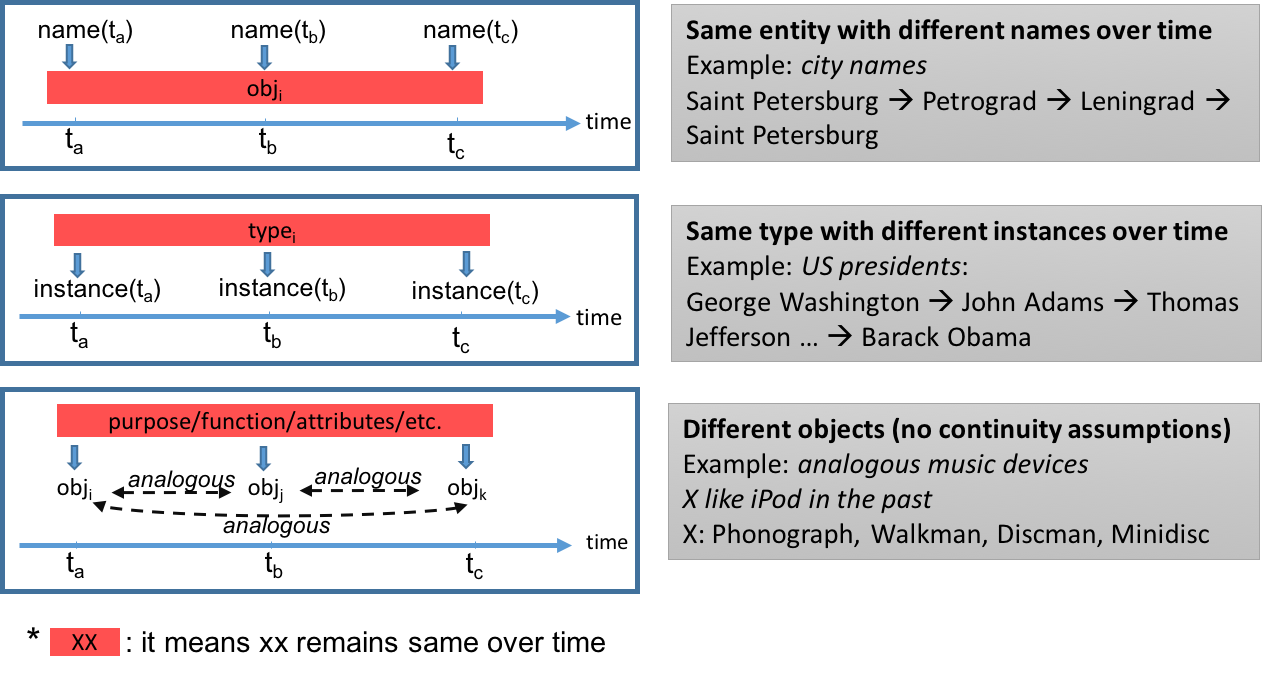
\includegraphics[width=0.8\textwidth]{figures/TAHMASEBI_Similarity_across_time3.png}
        \caption[Types of temporal analogs]{Conceptual view of three types ((2), (3) and (4) from the list above) of diachronic replacements.}
	\label{fig:across-time-sim}
\end{figure}



\citet{berberichbsw09} were probably the first to propose reformulating a query into terms used in the past in order to support user search within document archives spanning over long time periods. The task was defined as follows: given a query $q = {q_1, q_2,..,q_m}$ formulated using terminology valid at a reference time $R$, identify a query reformulation $q' = {q'_1, q'_2,..,q'_m}$ that paraphrases the same information need using terminology valid at a target time $T$. They measured the degree of relatedness between two terms used at different times through context comparison using co-occurrence statistics. A hidden Markov model was used for query reformulation; it considered three criteria of a good reformulation: \textsc{similarity}, \textsc{coherence}, and \textsc{popularity}. In particular, the similarity criterion requires that
$q_i$ and $q'_i$ have high degree of across-time semantic similarity, while coherence means that $q'_i$ and $q'_{i-1}$  should co-occur frequently at time $T$ to avoid combining unrelated terms. Finally, $q'_i$ should occur frequently at time $T$ to avoid unlikely query reformulations.
This approach may require recomputation each time a query is submitted because it needs a target time point for the query reformulation. 


\begin{sloppypar}
\citet{kaluarachchi2010incorporating} proposed that semantically identical words (or named entities) used at different time periods could be discovered using association rule mining to associate distinct entities with events. Sentences containing a subject, verb, and object 
are targeted and the verb is interpreted as an event. Two entities are then considered semantically related if their associated event is the same and the event occurs multiple times in a document archive. The temporally related term of a named entity is used for query translation (or reformulation) and results are retrieved appropriately with respect to specified time criteria. 
\end{sloppypar}

\citet{kanhabuan10} extracted time-based synonyms of named entities from link anchor texts in Wikipedia articles, using the full article history. Because of the limited time span of Wikipedia, they extended the discovered time of synonyms by using a burst detection method on the New York Times Annotated Corpus. Unfortunately, link information, such as anchor text, is rarely available and thus limits the method to hypertext collections. The authors evaluated the precision and recall of the time-based synonyms by measuring precision and recall in the search results rather than directly evaluating the quality of the synonyms found. 

\citet{tahmasebi2012neer} proposed a method called \emph{NEER} for discovering different names for the same named entities (e.g.,  \emph{Joseph Ratzinger} and \emph{Pope Benedict XVI}, \emph{Hillary Rodham} and \emph{Hillary Clinton}).
It relied first on detecting the periods that had a high likelihood of name changes and analyzed the contexts during the periods of change to find different temporal co-references of named entities. The key hypothesis was that this approach could capture both the old and the new co-reference in the same context. The underlying assumption was that named entity changes typically occur during a short time span due to special events (e.g., being elected pope, getting married or merging/splitting a company). Co-references were classified as direct and indirect. Direct co-references have some lexical overlap (e.g.,  \emph{President Obama} and \emph{Barack Obama}), while indirect ones lack any lexical overlap (e.g.,  \emph{President} and \emph{Barack Obama}). The proposed method first identified potential change periods via burst detection. Bursts related to an entity were found by retrieving all the documents in the corpus containing the query term, grouping them into monthly bins, and running the burst detection on the relative frequency of the documents in each bin. After NLP analysis, the method creates a co-occurrence graph of nouns, noun phrases and named entities from documents mentioning the input entity. The next step collapsed the co-references based on their lexical similarity and merged their contexts into co-reference classes. All terms in the context of a given co-reference class were then considered as candidate indirect co-references. 

\citet{tahmasebi2012neer} conducted experiments on the New York Times dataset using 16 distinct entities corresponding to 33 names and 86 co-references (44 indirect and 42 direct). Using a random forest classifier they achieved a precision of
90\% on known time periods and 93\% on found periods. 
The proposed method was later applied for query suggestion in search engines using temporal variants of a query \citep{holzmann2012fokas} and for detecting named entity evolution in the blogosphere \citep{holzmann2015named}.

As is typical, there is low overlap between contexts of temporal analogs, solutions that rely on measuring context overlap do not work well. Distributed word representations \citep[e.g.,][]{mikolov2013-distributed} 
can be useful for avoiding the problem of low context overlap. Given the representations trained on the distant time periods (typically, one derived from the present documents and another from documents published in the past), matching words across time could be done through transformation. This essentially means aligning relative positions of terms in the vector spaces of different time periods. \citet{zhang2016past} and later \citet{szymanski:2017} 
used a linear transformation matrix for finding translations between word embeddings trained on non-consecutive time periods for detecting temporal analogs. The inherent problem in this kind of approach is the difficulty of finding a large enough training set, given the variety of domains, document genres, and arbitrary time periods for finding temporal analogs. 
A simple solution proposed by \citet{zhang2016past} assumes that frequent and common terms in both time periods can be easily acquired and used for optimizing the linear transformation matrix. This idea is based on the observation that most frequent words are known to change their semantics across time only to a small degree \citep{hamilton-etal-2016-diachronic,pagel2007frequency,lieberman2007quantifying}. Initializing word embeddings using embeddings trained on previous time periods \citep{kim-etal-2014-temporal} is difficult given the potentially long gaps between the two periods on which the vector spaces were trained. The potential lack of data from the intermediate periods can be another problem.
The authors also successfully experimented with using terms that were computationally verified to have undergone little semantic variation across time as training instances for the transformation matrix. They did this by comparing sequentially trained word representations from consecutive time periods. Another improvement was the introduction of a local approach that relied on transforming automatically selected reference terms for a given query, which are supposed to ground the meaning of the query. Such transformed reference terms were then compared with the reference terms of candidate analogs, which had been generated by the previously described global transformation approach, with a linear transformation matrix. In other words, the global transformation approach was effectively extended with a method that locally constrains a query by transforming selected context terms called reference terms and then compares these terms with the ones of candidate analogs. The reference-to-reference term similarity measure relies not only on comparison of transformed vectors but also on comparison of transformed vector differences. The idea behind comparing vector differences was to capture the relation of a query (or a candidate analog) and its reference term.
Three methods were suggested for proposing the reference terms from candidate context terms: PMI, clustering, and hyperonym detection using shallow processing \citep{ohshima2010high} in an attempt to reflect the relevance, diversity, and generality of the reference terms, respectively.
Experiments were done on manually constructed ground truth data consisting of pairs of temporal analogs using precision at different cutoff points and mean reciprocal rank (MRR). The results showed that the local approach using reference terms selected from hyperonyms of a query (and of candidate terms) performed the best. The authors also demonstrated that correcting OCR errors by using a simple approach based on word embedding similarity and word frequency greatly enhances the quality of results. 

More recently, \citet{zhang:2017:tar:3132847.3132917} proposed using a set of transformation matrices based on different hierarchical clusters over the vocabularies in the two time periods. The thinking was that a single linear transformation matrix is insufficient for obtaining a good mapping between vector spaces of different periods. However, they found that using a series of matrices, such that each corresponded to a given hierarchical cluster of terms, and aggregating their results performed better.

\citet{orlikowski-etal-2018-learning} compared a number of models that rely on operations on word embeddings using nine different concepts on a corpus of Dutch newspapers from the 1950s and 1980s.
Following \citet{kenter2015ad}, the authors assumed the notion of diachronic concept change involving the core concept terms and characterizing concept terms. Based on that model, the characterizing terms are expected to change over time, while the surface forms of the core terms are assumed to stay the same. The problem of concept change at a particular time point is then reduced to the problem of predicting valid characterizing terms for a core concept term.

All the approaches proposed so far have relied on sense-agnostic solutions, essentially, mixing all the senses (or relying on the dominant sense). A future improvement would be to move into the direction of finding analogous terms with respect to their senses or topics/aspects (sometimes called viewpoints). For the example of the latter, consider \emph{Walkman} which corresponds to \emph{iPod} due to their similar function as a `music device', while \emph{PC} can be a reasonable analog when regarding \emph{iPod} as a `game player'. A queried term, for example, an entity, may contain multiple aspects and the temporal analogs could be different depending on the particular topic/aspect. In this regard, \citet{zhangwsdm} demonstrated a simple solution for an aspect-based temporal analog retrieval that takes additional terms as input to restrict the meaning of a user query to a particular viewpoint or aspect. The proposed solution also utilizes a neural network to realize non-linear term-to-term mapping. 

Furthermore, all the approaches, with the exception of the work by \citet{tahmasebi2012neer} and \citet{kaluarachchi}, need clearly specified time periods for comparison. While typically one of the periods represents the present (i.e., the time when a present-day user needs some information), the others can be any period in the past. It is, however, not always feasible to require users to specify specific periods for which temporal analogs need to be output. In many scenarios, it may be assumed that the user wants to know all the analogs from the past; hence, methods that can provide ranked results based on the agglomeration of results collected from different time periods should also be proposed. 

Outputting evidence for automatic explanation of term similarity is a related problem to estimating similarity across time. The approach proposed by \citet{zhang2016towards} relies on providing evidence of terms' similarity over time by outputting explanatory context terms and then extracting sentences that reveal the shared aspects between temporal analogs. For example, for the input query pair \texttt{ipod} and \texttt{walkman}, the pairs of explanatory terms could be \texttt{music}--\texttt{music}, \texttt{device}--\texttt{device}, \texttt{apple}--\texttt{sony}, \texttt{mp3}--\texttt{cassette}, and so on. Note that the input is now the pair of query terms instead of a single term, as it is in the temporal analog retrieval task, and the output is the ranked list of term pairs.
Term pairs are ranked based on their relevance to the input query pair as well as the intra-similarity between the pair elements and their relations to query terms (both similarities are computed after applying transformation).

For this, \citet{duan2019mapping} proposed an approach that uses joint integer linear programming and entity-oriented typicality analysis to generate multiple pairs of corresponding terms across time.


\citet{turney2019natural} used WordNet synsets and Google Books Ngram data to investigate the competition of words belonging to the same synset. The authors used a supervised learning approach (a naive Bayes classifier) to predict future leaders in the synset based on a range of features like word length, the characters in the word, and the historical frequencies of the word. The weaknesses of this approach are the assumption of the stability of synsets over time (the last two centuries) and inability to model words moving between synsets.

Finally, recent work by \citet{karjus2020communicative} demonstrated a simple way to find candidates of diachronic lexical replacements that is based on the comparison of word frequency changes and word semantics as represented by latent semantic analysis (LSA). Their competition model assumes that words which increase in frequency can substitute semantically similar words that experience decrease in their frequency around the same time. 


\section{Methodological issues and evaluation}\label{sec:method}
\subsection{Evaluation and hypothesis testing}\label{sec:evaltesting}
Today, it is considered more or less \emph{de rigueur} to accompany a proposed new method in computational linguistics with an \textsc{automatic, formal, quantitative evaluation}. This reflects a healthy development towards greater objectivity in reporting results, but it also comes with a greater responsibility on the part of the researchers to ensure that the evaluation metrics provide a true measure of the accuracy of the proposed method. 

Because of the vast amount of digitized information now available to us, there is currently a unique possibility to develop and test methods for detecting language change. However, the amount of data limits the possibility to use expert help and manual efforts in the detection phase. It is also a limiting factor in the evaluation phase as there are to date only a few existing, open datasets for diachronic conceptual change that can be used for evaluation purposes.\footnote{The SemEval-2020 Task 1 on unsupervised lexical semantic change detection presents a first large multilingual resource. The organizers report over 1,000 annotation hours and close to 20,000\,€ in costs for a human-annotated dataset for two time periods.} 

Specific to this problem is the grounding of diachronic conceptual change in a given corpus. When does a word appear for the first time with a new or changed sense in a given corpus? As a consequence, there are few automatic evaluation methods. Instead, there is a large variety of techniques, datasets and dimensions that are used in the existing literature. Most previous works have made use of manual evaluation while some have made use of WordNet for evaluation purposes. We argue that WordNet is not appropriate for evaluation for two main reasons. First, there is no indication in WordNet of \emph{when} a word's meaning changed or a new sense was added. Second, when datasets span hundred years or more, WordNet does not sufficiently cover the vocabulary or word senses in the dataset. The same holds for Wikipedia, which often covers changes but lacks time information \citep{holzmann2014insights}. In addition to the lack of data and resources for evaluation, there are no evaluation methods or metrics that have themselves been properly evaluated. 

Note that downstream applications, e.g., IR systems, can of course be evaluated in the normal way for such applications, which we will not describe here. Rather we will focus on methods for evaluating lexical change as uncovered by the methods surveyed here. A reasonable assumption would be that such an evaluation regime will also be useful -- at least in part -- for evaluating concrete downstream applications.

At least in the context of this literature survey, we would like to step back and see computational linguistics-style formal evaluation as part of a larger endeavor, as a central and necessary, but not sufficient, component of \textsc{(linguistic) hypothesis testing}. In particular, since the gold standard datasets which make up the backbone of our formal evaluation procedures are generally extremely expensive to create, there is an understandable tendency in our community to reuse existing gold standards to the greatest possible extent, or even re-purpose datasets originally constructed with other aims in mind.\footnote{Or even generate synthetic, simulated data assumed to faithfully reflect authentic data in all relevant aspects.} However, such reuse may be in conflict with some assumptions crucial to the original purpose of the dataset, which in turn could influence the results of the evaluation.

There are two central (typically tacit) methodological assumptions -- i.e. hypotheses -- made in the work described in the previous sections, and especially in work on diachronic conceptual change detection and classification (Sections~\ref{sec:wsch} and~\ref{sec:sdcd}):

\begin{enumerate}
    \item \textsc{applicability:} the proposed method is suitable for uncovering diachronic conceptual change.\label{hypo1}
    \item \textsc{representativeness:} the dataset on which the method is applied is suitable for uncovering diachronic conceptual change using this method.\label{hypo2}
\end{enumerate}

Since most current approaches are data-driven -- i.e. the data are an integral component of the method -- these two factors, while logically distinct, are heavily interdependent and almost impossible to keep apart in practice, and we will discuss them jointly here.

With a few notable exceptions, to which we will return below, there is also often a third tacit assumption:

\begin{enumerate}
    \setcounter{enumi}{2}
    \item \textsc{falsifiability and control conditions:} positive evidence is sufficient to show \ref{hypo1} and \ref{hypo2}.\label{hypo3}
\end{enumerate}

Assumption \ref{hypo3} comes at least in part from the common practice of evaluating diachronic conceptual change using lists of attested such changes, and is often logically wrong.

We will now take a closer look at these assumptions.

\subsection{Applicability and representativeness}\largerpage[2]
The first major difficulty when evaluating the results of diachronic conceptual change is the \emph{evaluation of a representation} $r \in R$ of a meaning of a word $w$ or a word sense $s_w$. When is $r$ a correct and complete representation of $w$ or $s_w$? Typically, this boils down to determining if a set of words, derived by clustering, topic modeling or from the closest words in a word space, indeed corresponds to the meaning of a word or word sense. In the case of multi-sense tracking, it is also important that the set of representations in $R$ are a complete representation of $w$ such that all its senses are represented in a correct way. The evaluation of individual word senses is analogous to the evaluation of word sense induction (see \citealp{agirre:semeval,navigli2012quick} for more details and an overview).  


Another related, more subtle, source of methodological muddles may be a misunderstanding of
what is being investigated. \citet{liberman-2013} points out that the
notion of ``word'' used in a paper by \citet{petersen-etal-2012} is
very far from how this term is understood by linguists, and the
purported statistical laws of vocabulary development as evidenced in
the Google Ngram dataset can be due to many other irrelevant factors,
foremost of which is varying OCR quality, but also ``tokenization'' as a faithful model of wordhood \citep{dridan-oepen-2012}.

Linguists have long recognized that ``language'' is a nebulous term, at best designating a convenient abstraction of a complex reality. This does not mean that any language sample should be considered equally representative, however. Especially corpus linguists have spent much intellectual effort on the question how to compile representative language samples, where it is clear that ``representative'' generally must be interpreted in relation to a specific research question. We mention this here, since we feel that it is important to be clear about what the changing entity is when we investigate lexical change. Given that linguists generally consider speech to be the primary mode of linguistic communication, are we happy investigating mainly written language, following a long tradition of ``written
language bias'' \citep{linell-2005} of general and perhaps especially computational
linguistics? Or given that the language should belong to every member of its speaker community, are we satisfied modeling the language of a select small social stratum \citep{henrich-etal-2010,sogaard-2016}? 
An interesting aspect of this discussion comes into play when employing pre-trained models like BERT: do the results live in the dataset being studied, or stem from the pre-trained model? Does this mean that the results are more general, though we typically have little say in what data is used in the pre-training phase?
Whatever the answers to these questions are, 
they need to be addressed.
 We should also recognize that to be able to use statistical inference from a corpus sample to the population as a whole, the sample must be random. Due to the above stated reasons, and many more, we cannot assume that written corpus data are ever a random sample of a language as a whole, and hence, we cannot use what we learn on a corpus to infer about the language in general \citep{koplenig2016}. To be able to reason about the language as a whole, we need many experiments from a wide range of sources to converge on the same conclusion. 
 
The second major difficulty concerns the \textsc{comparison of word senses} (via their approximations) over time. Because the word senses are approximations derived from time sliced corpora, the representations at different time points can be different without there being any actual sense change. Two factors can play a role:\largerpage[2]
	
	\begin{description}
	\item[Factor 1:] Imagine a set of contexts $C$ that contain word $w$. If we split $C$ into two random sets $ C_1$  and $C_2$, such that $C_1 \cup C_2 = C$, the representations of $w$ in $C_1$ and $C_2$ respectively will be different. Assuming that $|C_1|$ and $|C_2| \rightarrow \infty$ the difference in representation of $w$ for $C_1$  and $C_2$ should go to 0. However, this is rarely the case, since our datasets are finite in size and we see a difference in representations. Because we often use single genres of data, novels, news papers etc., we are likely to enhance this randomness effect; if a word is not used in a certain context due to missing underlying events, then the word sense will not be present. By using a mixed set of sources, we could reduce this effect. We see the same effect for representations of a word $w$ if $C_1$ and $C_2$ belong to two different time periods. 
		 
     Now, if $ C_1$  and $C_2$ represent two adjacent time periods, the task of diachronic conceptual change becomes to recognize how much of the difference in the representations of $w$  that is due to this randomness effect and how much is due to actual semantic drift. 
	\item[Factor 2:] Imagine that the representation of $w$ is a set of words $u_1, \ldots, u_n$ for time $t_i$ and $v_1,\ldots,v_n$ for time $t_j$. If each $v_j$ is a diachronic word replacement of $u_j$, then the entire representation of $w$ can be replaced between $t_i$ and $t_j$ without there being any change to the sense of $w$. While it is unlikely that all words are replaced between any $t_i$ and $t_j$, the risk of this effect increases the further apart the time periods. 
	\end{description} 

In other words, in order to argue that some instance of lexical variation constitutes
a case of diachronic conceptual change based on (massive) corpus evidence, it it
generally not enough to ascertain that the variation correlates with
different time slices of the dataset. It is also necessary to ensure that no other relevant variables are different between the time
slices. The original Culturomics paper \citep{michel2011quantitative}
has been criticized for not doing this, by \citet{pechenick-etal-2015}
and \citet{koplenig-2017b}, among others. This is also held forth as a
strong point of the smaller COHA dataset by its creator
\citep{davies2012expanding}. This pitfall can be avoided by devising control
conditions, but even so the purported diachronic effect may
conceivably disappear for other reasons as well, e.g.,  if some other
variable unintentionally correlates with time because of how the data
were compiled. An interesting example of this is the fact that two random, trending variables will have a moderate to high correlation despite being completely random \citep{koplenig2016population}. Here, the correlation stems from the fact that most diachronic corpora increase in volume over time and not necessarily from underlying semantic changes.

Another interesting reduction is the $n$-gram model, that automatically limits the amount of available information. To date, there has been little, if any, discussion in the diachronic conceptual change detection field to cover the effects of using $n$-grams rather than a full dataset with running text.\footnote{\citet[233]{gale-etal-1992-one} note that in their experiments on word-sense disambiguation, they ``have been able
to measure information at extremely large distances (10,000 words
away from the polysemous word in question), though obviously
most of the useful information appears relatively near the polysemous word (e.g., within the first 100 words or so).''} 
What happens when we remove words out of $n$-grams (which is the case when we only keep the $k$-most frequent words)? How many $n$-grams still have sufficient information left? What is the distribution of the remaining 1-, 2-, 3-, 4- and 5-grams after the filtering? This is particularly important when we consider those works that keep the $k$-most frequent words without normalizing over time, and hence have a modern bias among the kept words. If we start with equal samples over time, how many $n$-grams contribute over time?  

An important aspect of representativeness is language coverage. While it is certainly true that the studies surveyed here are on a
much larger scale than any historical linguistic studies heretofore
conducted, it is nevertheless misleading to characterize
traditional historical linguistic investigations as ``based on small and
anecdotal datasets'' \citep[2]{dubossarsky-2018}. This ignores the
combined weight of the diversity of active observations painstakingly
and diligently made over two centuries on many languages and language
families by a large number of scholars highly trained in linguistic
analysis, observations which are continually shared and discussed in
the professional literature of the discipline.
Against this is set computational 
work on massive textual (published) datasets largely confined to one language
-- the norm -- or a typologically and geographically skewed 
sample of a few languages. While such work undoubtedly will contribute valuable data points to our collective knowledge of lexical change, in order to make solid linguistic claims about this kind of language change, it would be desirable to conduct equivalent experiments on as many languages as possible \citep[see e.g., ][]{bender-2009,bender-2011,bender-2016}.

\subsubsection{Factors involved in evaluation of diachronic conceptual change detection}\label{sec:evaltechWSE}

\subsubsubsection{Granularity}
    
The first and most important factor that impacts evaluation is to determine the granularity on which to evaluate. Typically, change is evaluated with respect to change in the dominant sense of a word. That is, changes are not evaluated individually for all the senses of a word; instead, meaning change is evaluated for the form (text word or lemma), i.e. mixing all its senses. 
    Having a single representation per time period significantly reduces the complexity as it does not take into consideration what happens individually for each sense of a word. If a word has at most $s$ ($s\in S$) senses per time period over $t$ ($t \in T$) time periods, the number of unique senses is bound by $S\cdot |T|$. To compare all senses pairwise between time periods there are at most $|T|\cdot$S$^2$ comparisons needed. If we wish to evaluate the \textit{similarity graph} created by the senses in each time period, where edges correspond to similarity between two senses $s_i \in t_i$ and $s_j \in t_j$, there are $S^{|T|}$ possible paths. In comparison, for the single representation case, the number of unique senses are $|T|$ and the number of necessary comparisons is $|T|-1$  
    and there is only one path to evaluate. The number of time periods affect this complexity, and while some use yearly subcorpora, others use decades, reducing the time periods to compare by one order of magnitude. 
    
    
\subsubsubsection{Context}
What is considered the \textit{context} of a word differs largely between different works and is to some extent determined by the choice of dataset. A context ranges from 30 words surrounding $w$ \citep{sagi-etal-2009-semantic} to the word before and after \citep{gulordava-baroni-2011-distributional}. When the Google N-gram data is used, the context can be at most a window of 5 words (from 4 words before or after, the word $w$ being the first or last word, or 2 words before and after, the word $w$ being the 3rd word). For the pre-trained contextual embeddings of BERT, the sentence before, the target sentence and the sentence after are used as a context. What information is used as a context affects the representation. 

\subsubsubsection{Words included in the evaluation}	
An important part of evaluation is to determine which words to evaluate. Here two methods are employed; a set of pre-determined words, or the (ranked) output of the investigated method or methods.
	The former has the advantage of requiring less effort and reduces the need to conduct a new evaluation for each new run, with e.g., new parameters. The downside is, however, that the evaluation does not allow for new, previously unseen examples. Please note that using only positive examples can result in false conclusions: if we assume that the method always concludes change and is tested only on words where we expect change, it will be 100\% correct regardless of the choice of words. We believe that using negative examples to show the method's capacity to differentiate the positive and the negative examples is needed, and that the falsifiability assumption stated in Section~\ref{sec:evaltesting} is generally wrong.   
	
	\begin{description}
		\item[Pre-chosen testset]
		\begin{itemize}
            \item[]
			\item positive examples (words known to have changed)
			\item negative examples (words known to be stable)
		\end{itemize}
	\item[Output of algorithm]
		\begin{itemize}
            \item[]
			\item on the basis of a pre-determined measure of change (e.g., largest or smallest cosine angle between two consecutive time periods)
			\item randomly chosen set of words
		\end{itemize}
	\end{description}
	
		Most commonly, single words are used in evaluation, but it is becoming increasingly common to study the relation between (known) word pairs. That means, two words, typically one that is under investigation and one that represents the changed word sense, are evaluated with respect to their similarity over time. If a change takes place between the pair, this is used to confirm the hypothesis of diachronic conceptual change. Examples include (\emph{gay, homosexual}) that become more similar over time, or (\emph{gay, happy}) that become less similar over time. Both would confirm the same hypothesis about change in meaning for the word \emph{gay}. 
	Thus far, word pairs have always been used in a pre-chosen fashion. Choosing the word pairs that have the highest degree of change increases the computations by a polynomial factor. If we assume that there are $n$ words at time $t$, and worst case, a new set of words for each time period, then there are $(n^2)^t$ pairs available. Typically, the situation would be much less extreme and only a fraction of the vocabulary is exchanged per time period (the more, the further apart the time periods are).  Moreover, the reference term to be chosen for judging the changes of a target term should itself have stable meaning over time. For example, when tracking the similarity between \emph{gay} and \emph{happy} in order to detect or understand the sense change of the former, one implicitly assumes that \emph{happy} does not undergo significant semantic change over the time period of comparison.
	

\subsubsubsection{Evaluation technique} Evaluation can be conducted manually or automatically. Manual evaluation is done either with respect to intuition or pre-existing knowledge, or against one or more resources (dictionaries, encyclopedia etc.). Automatic evaluation is performed with respect to external resources, e.g., WordNet, or intrinsically where some evaluation metric is compared over time, e.g., statistically significant difference in the direction of the word vectors \citep{kulkarni2015statistically}. 

Evaluation of temporal analog search often follows IR style evaluation settings. For a given query a ranked list of analog terms is presented and metrics like precision/recall \citep{tahmasebi2012neer} or precision@1, precision@5 and MRR \citep{zhang2016past} are used based on the rate of correct analogs found in the top ranks.
	
\subsubsubsection{Change types included in the evaluation}	Evaluation for each word can be a binary decision; yes/no, there has been change, but it can also take the time dimension into consideration. The change is correct if it is found at the expected time point, or it is correct with a time delay that is measured. In addition to the binary decision, there are different change types (recall \tabref{tab:changetypes}, page~\pageref{tab:changetypes}, for a list of change types considered in this literature). The more types are considered, the more complex the evaluation becomes. With one exception, different change types are considered only for sense-differentiated methods, while word level change groups all changes into one class. Typically, change means a shift in the dominant sense of a word. E.g., Apple becomes a tech company and adds a dominant meaning to the word \emph{Apple}. However, its `fruit' sense is not gone but is very much still valid.\footnote{Note, however, that in written standard texts this ``change'' will partly be an artifact of preprocessing; lowercasing all text will increase the likelihood of conflating the common noun \emph{apple} and the proper noun \emph{Apple}. It is also in fact likely that the ``dominant'' sense of \emph{apple} is an artifact of the dominant modality and genre, and not a fact of language} Still, the change in dominant sense from `fruit/food' to `technology' is considered correct in a word level change setting. 
    

\subsubsubsection{Time dimension}
	The time span of the data makes a difference for evaluation. The further back in time, the harder it is to evaluate since there are fewer resources that cover the data (e.g., no reference resources such as dictionaries/wordnets/wikipedias for historical senses, etc.) and fewer experts to perform in-depth manual evaluation. The complexity is increased with the number of included time points. The more time points, the more complex the evaluation as there are more comparisons to evaluate. 
	
	The evaluation of time is an extremely complex matter; should it be done with respect to the outside world or the specific dataset under investigation? The complexity of the evaluation differs largely depending on the choice. To compare to the outside world means to make use of dictionaries and other knowledge sources to determine when a word came to existence, changed its meaning or added a sense (see \citealp{viola-frai.2020.00064} for example). The resource or resources used for this determination need not be tied to the dataset used and there are regional variations in uptake of new politics, technology, culture, etc., that in turn affect language use. 
    Newly coined terms, or senses can be due to an invention, one or a few influential sources, or an event and in such cases, be simpler to pinpoint in time. If the change, however, is due to a slow cultural shift or idiom that increases in popularity, it becomes very difficult to pinpoint the time of change. An analogy is that of fashion; when did the bob cut come into fashion? When the first ever person got such a haircut? Or the first celebrity showed it off on the red carpet (where is was better noticed and more likely to be duplicated)? Or when we can measure that a certain percentage of women had the hair cut as attested by e.g., school pictures or driver's licenses? In manual attestation of diachronic conceptual change it is common to discuss the explanatory power of a sense in a given time; however, that is hard to translate into a specific time point. A more or less arbitrary threshold can be used to translate an increasing (or decreasing) curve into a binary yes or no that can be used to specify a time point. 
    
    If we wish to evaluate with respect to the dataset, there is an added difficulty compared to the above. If the word itself is not novel, then it requires word sense disambiguation to find the first occurrence of a new or changed sense; when was a word used in a specific sense for the first time in the dataset?  If existing sense repositories are not available, the senses must first be induced and then assigned to individual instances of a word in the dataset which is, to some extent, to solve half of the diachronic conceptual change problem. In addition, the results might be different for each dataset, and hence it is a time consuming procedure that must be repeated. However, disregarding differences between datasets might penalize certain datasets, and hence experiments, compared to others, e.g., expecting an invention to appear in a dataset at invention time when in fact there might be a delay of  decades.  

For both methods there is a large difference between expecting to automatically find the first instance of change or expecting to find the change when it has gained enough momentum to be detectable by context-dependent methods.  An example of the differences in momentum but also the differences between datasets can be illustrated with the word \emph{computer}. An earlier common usage of this word was in reference to humans \citep{grier-2005}, but the `computing device' sense has been on the rise since the electro-mechanical analog computer was invented in the early 20th century and came to play an important role in the second world war, and its incidence has been increasing with the growing importance of digital computers. 
    The frequency of the word \emph{computer} in Google N-grams reaches over 0.0001\% in 1934 for the German portion, 1943 for the American English, and 1953 for the British English, meaning that a method evaluated on the latter dataset would be penalized by 20 years compared to one evaluated on a German dataset.\footnote{The word \emph{Rechner} was and is used in German as a synonym of \emph{Computer}.}    

Here we should also mention the sociolinguistic construct \textsc{apparent time} \citep{mague-2006} and a similar idea which informs much work in corpus-based lexicography. Apparent time rests on the assumption that crucial aspects of our linguistic repertoire reach a stable state at an early age, say around the age of 20, meaning that e.g., dialect studies can address diachronic development by recording age-stratified speaker samples synchronously, so that the language of a 70-year old is supposed to reflect -- in time capsule fashion -- current usage about 50 years ago. In a similar way, lexicographers assume that some genres are linguistically more conservative than others, and look for first appearances of new words or new word senses in news text rather than in fiction. Today, the intuition of dialectologists and lexicographers would conspire to single out social media texts as the main harbingers of lexical change \citep[e.g.,][]{fiser-ljubesic-2018}.
    
\subsection{Recommended evaluation procedure for diachronic conceptual change}
We recommend the following to be included in any evaluation procedure: 
\begin{enumerate}
\item \textit{Pre-chosen testset}: Compare the results for target words to words from the same frequency bin, or to the average behavior of all words, to reduce frequency bias, for both positive and negative words.
\item \textit{Grounding in the dataset}: Evaluate backwards referral to the original texts, e.g., by looking at randomly chosen $n$-grams or sentences, where the word under investigation occurs. 
\item \textit{Grounding in the outside world}: evaluate with respect to the outside world, e.g., dictionaries and encyclopedias. How well does the result correspond to the expected? The correspondence to the expected is particularly important if claims are made about language in general on the basis of results derived from the corpus. 
\item Consider conceptually and/or practically what happens if there is too little evidence in the text (for certain time periods) for a word: can meaning change be found?
\item Consider if the information found is present in the data at hand, or if it stems from the pre-trained models, and therefore possibly relates to a source outside of the dataset under investigation.
\item Can different change types be differentiated in theory? In practice? This question should be answered even if the method is not used for differentiated change types in the study. 
\item Can the time of change be found?
\item How does the method scale up to more time points? This relates in particular to those that evaluate change on a few, far apart time points.
\item Always declare and give grounds for evaluation judgments: \emph{Yes, we consider this to be correct because $\ldots$}, or: \emph{No, we consider this instance to be incorrect because $\ldots$}. 
\item Use proper falsifiability and control conditions.
\end{enumerate}

\subsection{Falsifiability and control conditions}\label{sec:falsifiability}

\citet{dubossarsky-etal-2017-outta} highlight the importance of falsifiability, 
by devising a simple ``sanity
check'', creating control conditions where no change of meaning
would be expected to occur. They reproduced previous studies which have purported to
establish laws of semantic change, two proposed by
\citet{hamilton-etal-2016-diachronic} and one proposed by themselves
\citep{dubossarsky2015bottom}, finding that in the control
conditions, they reported that sense change effects largely disappear or
become considerably smaller. They use the Google Books English fiction and sample 10 million 5-grams per year randomly from 1900--1999, each bin spanning a decade. Two control corpora are used, one randomly shuffles the 5-grams from all bins equally. The size of the vocabulary stays the same as in the original corpus, but most semantic change should be equally spread over the corpus, and hence not observable, or observable to a much lesser extent. A second control corpus is created by sampling 10 million 5-grams randomly from 1999, for 30 samples. Since all words are sampled from the same year, there should be no observable semantic change. Word representations are created using word counts, PPMI and SVD reduction of the PPMI matrix, and the three laws are evaluated on both the genuine corpus and the shuffled control corpus.  
%
All three laws were verified in the genuine corpus but also found again in the shuffled corpus. The three word representations were used with a cosine similarity measure on the second control corpus, the 30 samples drawn from 1999, and while the changed scores are all lower for the control corpus, they are significantly positive, showing that the proposed change measurements are affected by noise. Using analytic proofs, it is shown that the average cosine distance between a word's vectors from two different samples (using count-based representations) is negatively correlated with the word's frequency. 

The linguistic literature provides a wealth of fact and even more discussion about possible driving forces behind both linguistic
variation in general and linguistic change, typically accompanied by a
large number of empirical linguistic examples. As a minimal
methodological requirement, it would behoove authors proposing that a
computational method can bring new insight to the study of lexical
change in language, to demonstrate in a credible way that other kinds
of variation have been taken into account by e.g., the experimental
setup, which crucially includes choice of appropriate positive \emph{and negative} data. Especially claims that seem to fly in the face of established truths in the field should be extremely carefully grounded in relevant linguistic scholarship. For instance, \citet{hills-adelman-2015} report a finding that semantically, the vocabulary of American English has developed in the direction of greater concreteness over the last 200 years, which seems to go against a proposed generalization about semantic change, namely that concrete vocabulary tends to be extended with abstract senses  \citep[383]{urban-2015}. A closer scrutiny of the methodology of the study reveals some questionable details. Thus, the list of crowd-sourced concreteness ratings compiled by \citet{brysbaert-etal-2012} used in the study provides only one part of speech and one concreteness score per lemma, e.g. \emph{play} in this dataset is only a verb with a concreteness rating of 3.24 (on a 0--5 scale). In a follow-up study \citet{snefjella-etal-2018} approach the same problem using a considerably more methodologically sophisticated and careful approach, but which still raises some questions. Building on work by \citet{hamilton-etal-2016}, they compute decadal concreteness scores for the COHA corpus (for the period 1850--2000) based on a small set of seed words assumed to have stayed stable in extreme concreteness and abstractness over the whole investigated time period, and find the same trend of increasing concreteness in the corpus over time. As an anecdotal indication of the accuracy of their approach, they list the top 30 concrete and top 30 abstract (text) words that come out of their computation (e.g., \emph{muddy, knives} vs. \emph{exists, doctrine}) and also report statistical correlations between the computed scores and several sets of human ratings, including those of \citet{brysbaert-etal-2012}. However, looking at the scatterplots provided by  \citet[6]{snefjella-etal-2018}, it is clear that the computed scores inflate concreteness compared to the human ratings, and in particular at the more abstract end of the concreteness range.\footnote{This does not in itself invalidate their result, of course. If this tendency is consistent over time, we are still seeing a diachronic increase in concreteness of the same magnitude that they report.} Further, if we POS tag the results\footnote{Their resulting data are available in their entirety at \url{http://kupermanreadlab.mcmaster.ca/kupermanreadlab/downloads/concreteness-scores.zip}} we note that many function words (e.g., determiners and prepositions) come out as highly concrete (e.g., \emph{the} is very close to \emph{muddy} for some of the decades), whereas they cluster consistently at the abstract end in the human ratings. The results reported by \citet{hills-adelman-2015} and \citet{snefjella-etal-2018} are very interesting to a historical linguist and deserve further study, but their studies should be replicated, with clear control conditions informed by awareness of historical linguistic facts, before any secure conclusions can be drawn.


\iffalse
\subsection{Datasets and testsets}\label{Evaluation_diach_replacement}
We briefly discuss here some of the datasets that have been used in the literature (or that could be used) for automatic evaluation of lexical and semantic change over time. The list is not exhaustive. 

Large scale data is the basis for effective and reliable word analysis. The largest available historical corpora\footnote{We follow general practice in the computational linguistic literature and use the term ``corpus'' even about datasets such as the Google Books Ngram dataset, which are not strictly speaking corpora in the corpus linguistic sense, in other words are not composed of complete texts.} with a comprehensive representation of several languages in the past are probably the \textbf{Google Books Ngram datasets}, which are available online.\footnote{\url{http://storage.googleapis.com/books/ngrams/books/datasetsv2.html}} The English datasets, for example, cover about 5\% of all books ever published. The total size of Ngram lists ($n={1,2,3,4,5}$) is quite large (about 0.3 trillion words), which typically necessitates provision of effective and scalable methods. The data are organized as ngram counts by every year and are available for several languages including English, French, Spanish. There are also some specialized English corpora available, such as American English, British English, and English Fiction. Google Books Ngram datasets come in two versions: version 1 (compiled on July 2009) and version 2 (compiled on July 2012).
Due to the scarcity of available books, the data for the period before the 19th century tends to be sparse (e.g., it is estimated that only about 500,000 books were published in English before the 19th century). In addition, there is the potential for a high number of OCR errors for the texts written in earlier centuries due to deterioration in the quality of paper, non-standard fonts, many spelling variants, and so on. According to the dataset creators, the rate of OCR errors is however limited, as $n$-grams that appear less than 40 times across the corpus have been removed. Independent analysis \citep{pechenick-etal-2015} has highlighted a number of limitations of the datasets. 
One concern was that they are increasingly dominated by scientific publications rather than by popular works. Nevertheless, Google Books Ngrams have been used frequently for not only diachronic linguistics but also for culturomics studies aiming to capture societal and cultural changes over time \citep{michel2011quantitative}.

Another corpus commonly used for diachronic conceptual change analysis is the \textbf{Corpus of Historical American English} (COHA) developed by Brigham Young University (BYU) \citep{davies2012expanding}.\footnote{\url{https://corpus.byu.edu/coha/}} Unlike the Google Books Ngrams datasets, COHA has been compiled with decade-level granularity. An important advantage of COHA is that it is based on a stable distribution of diverse document genres for each decade. The document genres (e.g.,  fiction, magazine, newspapers) were chosen according to the Library of Congress categorization scheme.\footnote{\url{http://www.loc.gov/catdir/cpso/lcco/}} COHA contains over 400M words given as $n$-grams ($n={1,2,3,4}$) collected from about 107K documents published from the 1810s to the 2010s. Each ngram is associated with its count in every decade. Part-of-speech tags are also available. According to COHA creators, the corpus is 99.85\% accurate,
which means, on average, there is one error for about every 500--1000 words. COHA is also available as a conventional full-text corpus. \footnote{\url{https://www.corpusdata.org/}}

The two above-mentioned datasets are substantially different. The Google Books Ngrams datasets have been compiled using all the books digitized through the
Google Books initiative. In contrast, COHA contains carefully selected texts and it is characterized by a stable rate of different document genres across decades. However, many rare words are not present in COHA making it useful only for the analysis of relatively common terms. On the other hand, the Google Books Ngrams datasets are more effective in this regard, given their large size. 
The weakness of both datasets is relatively short text window used for computing $n$-grams (up to 5 and 4 words), which makes it impossible to capture long distance word dependencies as also noted by \citet{tang-2018}, unless one uses the full texts. Finally, pre-trained, downloadable word embeddings for historical text are available \citep{hamilton-etal-2016-diachronic} based on the Google Books Ngrams and partially on COHA.\footnote{\url{https://nlp.stanford.edu/projects/histwords/}}

The \textbf{Corpus of Contemporary American English} (COCA) \citep{davies2010} is another balanced corpus from BYU.\footnote{\url{https://corpus.byu.edu/coca/}} As it spans a much shorter time frame (1990--2017), it could be used for analyzing short-term and recent changes in word meaning. The dataset comprises more than 560 million words, and 20 million words per year. COCA has been compiled from spoken, fiction, popular magazines, newspapers and academic texts.

\textbf{DiAchronic TExt corpus} (\textbf{DATE}) covers the years between 1700 to 2010, combining data from the COHA corpus, the training data from SemEval-2015 Task 7: Diachronic Text Evaluation \citep{popescu2015semeval} and the portion of \textbf{The Corpus of Late Modern English Texts, version 3.0}\footnote{\url{https://perswww.kuleuven.be/~u0044428/clmet3_0.htm}}, (\textbf{CLMET3.0}) \citep{diller2011european}. 
CLMET3.0 is a collection of public domain texts obtained from various online archiving projects; it contains about 34 million words and covers the period from 1710 to 1920, divided into three periods.

The \textbf{TIME corpus}\footnote{\url{https://corpus.byu.edu/time/}} was generated from new articles published in a single source: TIME magazine from 1923 to 2006.
The 275,000 articles processed provided 100 million words of text. Other similar collections of a single source are: the \textbf{Times Digital Archive} \footnote{\url{https://www.gale.com/uk/c/the-times-digital-archive
}} (from 1785 to 2012) and the \textbf{New York Times Annotated Corpus} \footnote{\url{https://catalog.ldc.upenn.edu/ldc2008t19}} (from 1987 to 2007). 

Among the other corpora\footnote{More examples of available corpora are also listed in: \url{http://davies-linguistics.byu.edu/personal/histengcorp.htm}} worth noting are the \textbf{Lampeter Corpus of Early Modern English Tracts},\footnote{\url{http://clu.uni.no/icame/manuals/LAMPETER/LAMPHOME.HTM}} the \textbf{Corpus of Early English Correspondence} (\textbf{CEEC}),\footnote{\url{http://clu.uni.no/icame/manuals/CEECS/INDEX.HTM}} the \textbf{Diachronic Part of the Helsinki Corpus of English Texts},\footnote{\url{http://clu.uni.no/icame/manuals/HC/INDEX.HTM}} and the \textbf{Diachronic Corpus of Present-Day Spoken English} (\textbf{DCPSE}).\footnote{\url{http://www.ucl.ac.uk/english-usage/projects/dcpse/}}
\textbf{Project Gutenberg}\footnote{\url{http://www.gutenberg.org/}}, one of the oldest digital libraries, was founded in 1971 and provides over 50k digitized books from the public domain in plain text and other formats. 
 \textbf{HathiTrust}\footnote{\url{http://www.hathitrust.org}} is a large-scale collaborative repository containing digital content from research libraries and other sources in collaboration with Google Books and Internet Archive projects. The library offers over 13 million books via full text search. \textbf{Early English Books Online (EEBO)}\footnote{\url{https://corpus.byu.edu/eebo/}} is a collection of texts created by the Text Creation Partnership, which contains 755 million words in 25,368 texts from the 1470s to the 1690s. \textbf{CLARIN ERIC}, a large European research infrastructure based on language technology and language resources, has published a list of 70 historical corpora. It covers a large number of (primarily European) languages.\footnote{\url{https://www.clarin.eu/resource-families/historical-corpora\#list-of-publications-on-historical-corpora}}
The \textbf{Internet Archive}'s text collection\footnote{\url{https://archive.org/details/texts}} contains more than 15 million freely downloadable digitized texts in different languages (mainly in English) amassed from various libraries and cultural heritage institutions. 

Court rulings, decisions, and criminal trials make up a genre of resources that has survived in recognizable form through centuries. For example, \textbf{Corpus of US Supreme Court Opinions}\footnote{\url{https://corpus.byu.edu/scotus/}} contains around 130 million words from 32k decisions of USA Supreme Court dating from the 1790s until the present. 
The \textbf{Proceedings of the Old Bailey}\footnote{\url{https://www.oldbaileyonline.org/}} (1674 -- 1913) are a fully searchable body of the records of close to 200,000 criminal trials at London's central criminal court providing a unique glimpse into the lives of non-elite people in London over a relatively long time. 

Other resources can be more domain-specific. 
Such datasets can be used to track sense changes of terms in specialized domains.
For example, \textbf{Hansard}\footnote{\url{https://www.hansard-corpus.org/}} is a specialized corpus containing almost every speech delivered in the British Parliament from 1803 to 2005 (over 7.5 million texts). Besides the access to the full texts,\footnote{\url{http://www.hansard-archive.parliament.uk/}} users may also search within the corpus.\footnote{\url{https://www.hansard-corpus.org/x.asp}}
 \textbf{Medline}\footnote{\url{https://www.ncbi.nlm.nih.gov/pubmed/}} is a repository containing articles in medicine and related fields, published from 1950s on. The \textbf{Association of Computational Linguistics (ACL) Anthology} corpus \citep{radev2013acl}, which spans the period from 1965 to 2013, contains scientific papers published in ACL venues. \textbf{Amazon Product Reviews}\footnote{\url{https://snap.stanford.edu/data/web-Movies.html}} and \textbf{Amazon Movie Reviews}\footnote{\url{https://snap.stanford.edu/data/web-Movies.html}} are other examples of specialized datasets; they cover 18 and 10 years, respectively.

Thesauri are other resources that can support diachronic analysis over time. One example is the \textbf{Historical Thesaurus of English}.\footnote{\url{http://historicalthesaurus.arts.gla.ac.uk/guide/}} It contains nearly all words that were recorded from Old English period until the present. The thesaurus was created based on the Oxford English Dictionary (OED) data as well as on the second edition of the Thesaurus of Old English. It contains the records of word use with the date information as well as style, frequency, or geographical labels. Word synonyms are arranged in chronological order based on their first recorded date. As words' last recorded dates are also sometimes available, this resource can be used for finding obsolete words or obsolete meanings of presently used words. \textbf{Roget's Thesaurus} \citep{roget-1852} is another widely used English-language thesaurus, which has appeared in numerous editions and variants since its first appearance in the mid-19th century. Its past editions offer unique opportunities to explore lexical information as recorded by researchers in the past.
We note that, to the best of our knowledge, there is no ready lexical reference system for historical language that would be similar to WordNet \citep{miller1990introduction} in which data on historical senses of words are represented in a structured format using synonym sets and their relations. 


\subsubsection{Testsets for lexical replacement}
When it comes to finding diachronic replacements or estimating the across-time similarity, any document collections with a sufficiently long time span and large enough size can be used as underlying datasets. For example, the \textbf{New York Times Annotated Corpus} (NYT) and the \textbf{Times Digital Archive} have been used for these purposes. 

Test sets for both of these datasets have been created for selected time periods \citep{tahmasebi2012neer, zhang2016past}. \citet{tahmasebi2012neer} introduced a test set\footnote{\url{http://tahmasebi.se/project/neer/}} composed of 86 co-references that correspond to 33 distinct entities that had changed their names over time (e.g.,  \emph{Pope Benedict XVI}, \emph{Cardinal Joseph Ratzinger}). All the terms exist in NYT Corpus and have at least 5 occurrences during the year when the name change occurred. The authors provided also an extended version of the test set containing named entity pairs whose name change happened outside of the time span of the NYT corpus or that occur just a few times in the text.

The short-term test set\footnote{\url{http://www.dl.kuis.kyoto-u.ac.jp/~adam/temporalsearch_short.txt}} for NYT that was used by \citet{zhang2016past}, contains 52 pairs of term analogs. The terms were selected from three equal size time periods: [2002,2007], [1992,1996], and [1987,1991]. The authors have also provided an extended version\footnote{\url{http://www.dl.kuis.kyoto-u.ac.jp/~adam/temporalsearch_short_extended.txt}}\citep{zhang:2017:tar:3132847.3132917} which in total has 225 term pairs for the two time periods compared [2002,2007] and [1987,1991] and 100 term pairs for [2002,2007] and [1992,1996]. Three types of entities are represented: persons, locations and objects. Persons include presidents,
prime ministers and chancellors of the most developed and populous countries (e.g.,  USA, UK, France) as well as the names of
popes and FIFA presidents. Locations include names of countries or cities (e.g.,  \emph{Czechoslovakia}, \emph{Berlin}) that have changed their names over time, split into several countries, merged into another political system, or became new capitals. Finally, objects contain terms denoting devices (e.g.,  \emph{iPod}, \emph{mobile phone}, \emph{dvd}), societal phenomena (e.g.,  \emph{email}), companies/institutions (e.g.,  \emph{NATO}, \emph{Boeing}) or other objects (e.g.,  \emph{letter}, \emph{euro}).
The authors also provided a long-term test set\footnote{\url{http://www.dl.kuis.kyoto-u.ac.jp/~adam/temporalsearch_long.txt
}} for the Times Digital Archive, which is composed of 400 query pairs collected from diverse time periods covering the 20th century. Due to sparse data in the past, the time periods in the more distant past are longer than the ones in near past so that all contain data of more or less similar size, which is needed for effective word embedding training.

\subsubsection{Data Quality}

Determination of word senses and their changes must be done on high quality datasets that are representative of the language used at particular time. We briefly discuss here some of the issues related to the choice of datasets.

There is an over representation of English datasets in literature. This is a result of easily available datasets, with sufficient volume and time span. However, the current bias towards English, indicates the need for evaluating and developing methods for other languages as well. Not all languages have such volumes of digitized historical texts, which means that despite the shift towards methods for tackling large scale data, we need to, simultaneously, keep investigating methods that can detect change from small scale or fragmentary data.
Moreover, few existing datsets are of a scale large enough to permit investigation of less common words. This is especially critical for earlier periods for which the data tends to be sparse and subject to more OCR errors.

The representativeness of datasets is another issue that determines if one can accurately represent the language used at a particular time. Naturally, due to the way they are created, mamy corpora tend to reflect written language, which may differ significantly from spoken language (especially, considering that the skills of writing and reading were often the privilege of narrow groups in the past). Another concern is the need to balance the different document genres over time as well as the geographical distribution from where the content is collected. In general, good dataset representativeness means maintaining, as much as possible, realistic balance over many text attributes including document genre, topic, originating location, author's age, gender, social position, among others. As preparing representative datasets is often difficult, any obtained results should at least be compared over two or more corpora, especially ones that have different or complementary
characteristics.

We note that the results derived from a single dataset without full coverage of a language, provide a picture of the language use in that particular dataset. Such insight is an excellent resource for archival search and help in interpreting the content of that particular dataset. While results of this kind do not offer a complete view of what has happened in a language, they do offer a complementary view. Results derived from, for example, a dataset containing texts created solely by religious institutions might not correspond to other society segments (e.g., peasants, merchants, or even females), but will offer us a view of a historical variant of a language, and can possibly offer insights into the general language as well. However, important when presenting results is to reason about representativeness of the data, and to not overstate the results.  
\fi

\section{Summary, conclusions and research directions}\label{sec:summary}

We summarize below the main observations of our survey. 

First of all, we note that the field has grown rapidly in the last few years, resulting in a variety of techniques for lexical semantic change detection, ranging from counting approaches over generative models to neural network based word embeddings. The state of the art is represented by methods based on word embedding techniques. However, most of these approaches are sense-agnostic, effectively focusing on the mixture of word senses expressed by a lexeme. Although some claim that their methods utilize the dominant word sense, they use each occurrence of the lexeme or word form without detecting if it is indeed representing the dominant sense or not. 

Another common shortcoming is that only a few approaches propose techniques capable of analyzing semantic change in words with relatively few occurrences. The amount of data for low-frequency words may be insufficient to construct reliable hypotheses using standard methods. Dynamic embeddings seem to offer a more suitable alternative with respect to small datasets. 
When moving to sense-differentiated embeddings, most likely even more data is needed, and the dynamic embeddings can be a path forward.
In relation to this, a common restriction of the discussed methods is that they work on a vocabulary common to all the investigated time periods and make use of the $k$ most common words. In some cases, the word frequencies are first normalized per year to avoid a dominance of modern words (since the available digital datasets grow in size over time). Still, this means that only words extant in the datasets over the entire time period contribute to the analysis, both in that they are the only words for which change can be detected, but also because they cannot contribute to the meaning of present words. A word like the Old Swedish legal term \emph{bakvaþi}, meaning `the act of accidentally stabbing someone standing behind you when taking aim to swing your sword forward', is only valid for a period and then disappears from our vocabulary. By ignoring this word, we will not capture any changes regarding the word, which has a very interesting story, but we also prevent it from contributing to the meaning of any of our other $k$ words.

In addition, since most of the corpora are not first standardized with respect to spelling variation, many common words are ignored only because their spelling has changed over time. For example, \textit{infynyt, infinit, infinyte, infynit, infineit} are all historical spelling variations used at different times for the word now spelled \textit{infinite} \citep{oed}. To properly address the problem of discovering and describing language change, we need to combine spelling variation, sense variation and lexical replacements in one framework.

Next, while a sense change may be successfully detected \emph{as a diachronic process}, determining the exact time point of semantic change requires the formulation of auxiliary hypotheses about the criteria to be used for determining this. Such criteria are obviously dependent on the available data. For most historical periods we have only texts typically produced by a small and skewed sample of the entire language community. Will thresholds of occurrence in historical texts faithfully reflect underlying change points? 

When it comes to evaluating methods and systems, there is a general lack of standardized evaluation practices. Different papers use different datasets and testset words, making it difficult or impossible to compare the proposed solutions. Proper evaluation metrics for semantic change detection and temporal analog detection have not been yet established. Furthermore, comparing methods proposed by different groups is difficult due to varying preprocessing details. For example, filtering out infrequent words can impact the results considerably and different papers employ different thresholds for removing rare words (e.g., some filter out words that appear less than 5 times, others less than 200 times). We suggest the use of SemEval-2020 Task 1 \citep{schlechtweg-etal-2020-semeval} and corresponding, standardized sources and tasks that facilitate comparability, and encourage authors to release their code for better reproducability and model comparison. 

Only a few proposals seem to allow for automatically outputting evidence of change to explain to users the nuances of the sense change and to provide concrete examples. Change type determination by automatic means is one step towards this.  Related to this is the need for more user-friendly and extensive visualization approaches for diachronic conceptual change analysis given its inherent complexity (see \citealt{chapters/10}). One should keep in mind that many researchers in, for example, the humanities will not accept tools that require programming skills on the part of the user, yet they require tools that are powerful enough to address non-trivial questions and to enable in-depth investigation.

The issue of interdependence between semantic changes of different words is also an interesting avenue of research. Most of the surveyed approaches focus on a single word, with only a few authors proposing to view sense change of a target word in relation to another reference word. Future approaches may take entire concepts or topics for investigation so that sense fluctuations of a given word would be seen in the context of changes of other words that may represent the same concept, the same topic or may be semantically related in some other way. Rather than analyzing diachronic conceptual change independently from the changes of other words, a more exhaustive approach could consider also senses of words belonging to an intricate net of word-to-word inter-relations. This could result in a more complete and accurate understanding of why and how a given word changed its sense.

Finally, we note that the linguistic study of semantic change has
traditionally been pursued in the context of single languages or
language families, and on limited data sets. In particular, nearly all the proposed approaches in the computational literature reviewed here are applied to English data only, due to the dominant position of English in various respects, which is reflected not least in the limited availability of datasets in other languages. Notably, the need for diachronic corpora in other languages than English has also been emphasized in the mentioned survey by \citet{tang-2018}.
Even if some ``laws'' of semantic change have been suggested \citep[e.g.,][]{wilkins,traugott2001regularity}, and general classifications of semantic changes into types have been proposed \citep[see][]{urban-2015}, albeit also questioned \citep[see][]{fortson-2003}, the field is still underdeveloped with regard to its empirical basis. For example, it would be necessary to carefully consider whether the underlying corpus is indeed representative of the given language, and does not introduce any bias towards a particular region, gender, social group, and so on, before making any general claims. Approaches that rely on corroborating results using different datasets could be helpful here, especially if informed by a solid knowledge of linguistic methodology and applied to a significant number of genetically, typologically and geographically diverse languages, allowing for both extension and validation of databases such as the \emph{catalogue of semantic shifts} manually compiled by \citet{zalizniak-etal-2012}. How applicable the investigated methods will be to other languages is ultimately an empirical matter, but we see no reasons not to be optimistic in this regard.


In view of the above finding, we list below several recommendations: 

\begin{itemize}
\item When showing and discussing results in a paper, the authors should provide their viewpoint and justification thereof, whether these results are correct or not, and why. 

\item Always use some sort of control, be it time-stable words or a control dataset, since in isolation, numbers are not sufficient.

\item While there have been several methods proposed so far for automatically detecting semantic change, still there are no solutions for automatically generating the ``story of the word''. Such story-telling would help to concisely explain how the term changed, perhaps giving also a reason for the change (e.g., a new invention). Automatically detecting the type of change could be seen as the first step towards this goal.
\end{itemize}



\section*{Acknowledgments}
Thanks go to the Center for Digital Humanities, University of Gothenburg and to Kyoto University. A first version of this work was written while Nina Tahmasebi was employed at CDH. Adam Jatowt was employed by Kyoto University when the first version was completed. This work has in part been funded by the project \textit{Towards Computational Lexical Semantic Change Detection} supported  by the Swedish Research Council (2019–2022; contract 2018-01184), the project \emph{South Asia as a linguistic area?} funded by the Swedish Research Council (2015--2020; contract 2014-00969), and \emph{Nationella språkbanken} (the Swedish National Language Bank), a research infrastructure jointly financed by the Swedish Research Council (2018--2024; contract 2017-00626) and the ten partner institutions. In
addition we are grateful for the strong and enduring commitment that the
University of Gothenburg, its Faculty of Humanities, and its
Department of Swedish have shown to our R\&D unit Språkbanken Text for
almost 50 years. 
The authors would also like to acknowledge Dominik Schlechtweg, Haim Dubossarsky, and Simon Hengchen for fruitful discussions and insights.  
The authors wish to thank the Department of Literature, History of Ideas, and Religion at the University of Gothenburg for providing financial support for language editing services.

\section*{Abbreviations}
\begin{tabbing}
EVALITA\hspace{1em}\= Evaluation of NLP and Speech Tools for Italian\kill
ACL \> Association for Computational Linguistics\\
BNC \> British National Corpus\\
DBSCAN \> Density-based spatial clustering of applications with noise\\
DSG-f \> dynamic skip-gram with filtering\\
DSG-s \> dynamic skip-gram with smoothing\\
EVALITA \> Evaluation of NLP and Speech Tools for Italian\\
LDA \> latent Dirichlet allocation \\
LSA \> latent semantic analysis\\
MRR \> mean reciprocal rank\\
NLP \> Natural Language Processing\\
NMI \> normalized mutual information\\
OCR \> optical character recognition\\
OED \> Oxford English Dictionary\\
PMI \> pointwise mutual information\\
POS \> part-of-speech\\
PPMI \> positive pointwise mutual information\\
SGNS \> skip-gram with negative sampling\\
SVD \> singular value decomposition\\
ukwac \> UK web archive\\
WSI \> word sense induction
\end{tabbing}

{\sloppy\printbibliography[heading=subbibliography,notkeyword=this]}
\end{document}
